\chapter{Desarrollo de la Solución}
En el presnete capítulo se describe las herramientas y procesos de desarrollo del modelo de Deep Learning.

\section{Determinación y evaluación de alternativas de solución}

En esta sección se presentarán las arquitecturas base CNN y ViT que se usarán en el entrenamiento de los modelos de Deep Learning para la tarea de clasificación de nódulos tiroideos a través de imágenes de ultrasonido. Además, también se introducirá la idea de modelo híbrido que junta las capacidades de extracción de características de los CNN con la actualmente popular arquitectura ViT.

En el grupo de modelos CNN, se tiene en primera instancia a la arquitectura VGG16, ya presentada anteriormente en el Capítulo 2.Este modelo posee 16 capas de profundidad junto con un tamaño de 3 x 3 en los filtros. Se ha reconocido que VGG16, y las arquitecturas VGGNet en general, poseen una alta capacidad de generalización, lo cuál lo vuelve ideal para tareas de clasificación distintas a los que originalmente fue entrenado. \parencite{pr_simonyan2015vdcn}

En segundo lugar, también parte del grupo de modelos CNN, se tiene a ResNet 50, también ya presentado inicialmente en el Capítulo 2. Esta arquitectura introdujo el concepto de redes residuales que permitieron obtener de manera más optimizada un mayor desempeño en arquitecturas de alta profundidad. \parencite{pr_he2016deepres} La versión de ResNet usada en esta investigación fue la de 50 capas de profundidad.

En el conjunto de modelos ViT, el usado en la presente investigación fue la ViT-Base con patch de tamaño 16 x 16.

Los modelos ViT también ya fueron presentados en el Capítulo 2.

Esta arquitectura, basada en los originales Transformers, ha demostrado tener mejor desempeño en tareas de clasificación comparado a los modelos basados en CNNs, aunque ciertamente con una mayor necesidad de datos de entrenamiento.

En la Figura \ref{2:fig206}, ya se muestra la forma de la arquitectura del modelo ViT. Cabe volver a resaltar que la versión del modelo ViT utilizado es el Base que consta de 86 millones de parámetros y recibe patch de tamaño 16 x 16.

Finalmente, el último modelo presente en la investigación es uno que combina la capacidad de los CNN y los ViT para obtener un modelo híbrido.

Este modelo utiliza al CNN como backbone que alimentará los features extraídos en forma de patch de tamaño 1 x 1 al modelo ViT. Para lograr esto se es necesario quitar el cabezal clasificador de la arquitectura CNN, pues esta tarea ya será desarrollada por el propio ViT.

Debido a las limitaciones de tiempo y recursos, solamente se desarrollará dos modelos híbridos con aquellos CNN de mejor desempeño en los entrenamientos iniciales.

Cabe destacar que este modelo híbrido fue inspirado por el trabajo presentado por \cite{pr_JERBI2023autoclassViTGAN}. A continuación se presenta la Figura \ref{4:fig101}, donde se muestra la arquitectura híbrida.

\begin{figure}[H]
	\begin{center}
		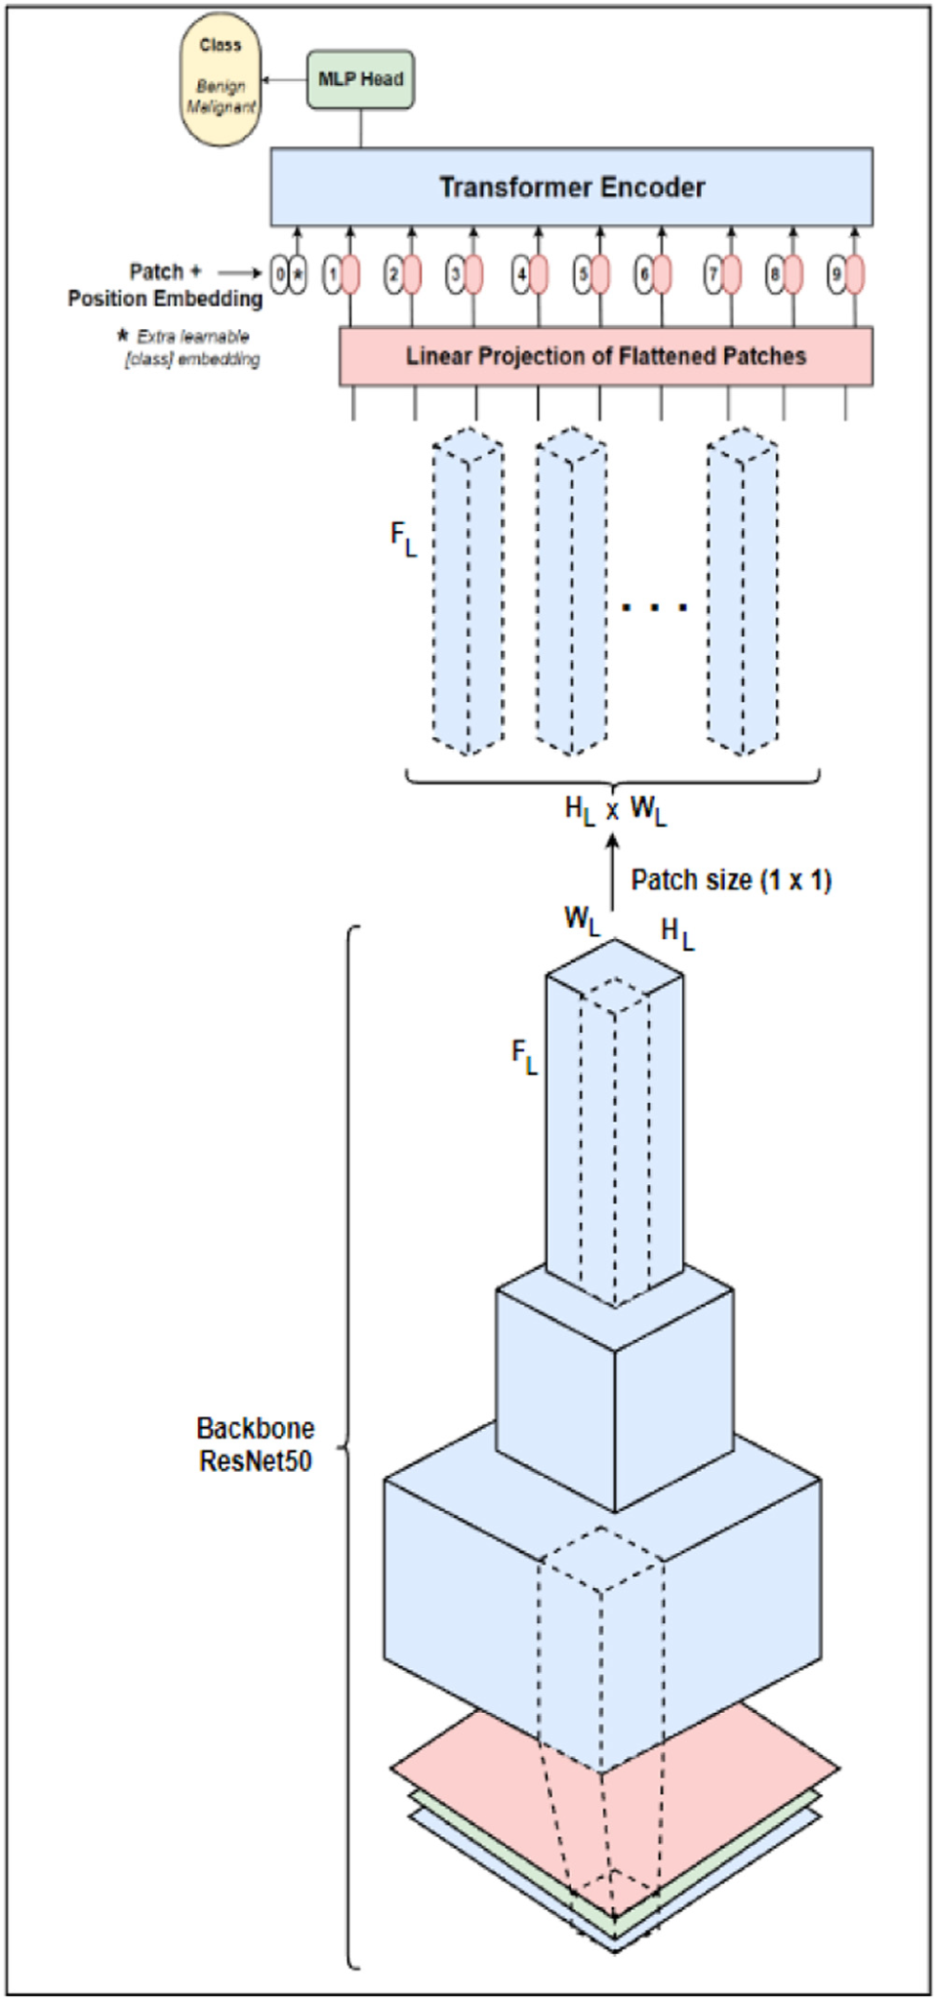
\includegraphics[width=0.60\textwidth]{4/figures/hybrid_arc.png}
		\caption[Arquitectura híbrida CNN + ViT]{Arquitectura híbrida CNN + ViT. \\
		Fuente: \cite{pr_JERBI2023autoclassViTGAN}. \textit{Automatic classification of ultrasound thyroids images using vision transformers and generative adversarial networks}.}
		\label{4:fig101}
	\end{center}
\end{figure}

\section{Propuesta solución}

\subsection{Planeamiento y descripción de Actividades}

La metodología descrita en el capítulo anterior consta de tres etapas principales: adquisición de datos, preprocesamiento de los datos y la aplicación de Deep Learning; es decir, el entrenamiento de los diferentes tipos de algoritmos. En la siguiente parte de esta investigación se procederá describir las actividades necesarias para desarrollar y completar cada una de estas etapas para, finalmente, obtener los resultados de cada uno de los modelos entrenados.

La metodología inicia con la adquisición del conjunto de datos necesario para realizar el entrenamiento de los modelos de Deep Learning. Este consta de las siguientes actividades.

\textbf{Actividad 1: Buscar y revisar bases de datos sobre imágenes de ultrasonido de nódulos tiroideos}
\\
En esta actividad se investigarán y analizarán aquellos conjunto de datos que cumplan con las características básicas requeridas: poseer imágenes de ultrasonido de nódulos tiroideos benignos y malignos.

\textbf{Entregable:} Diversos conjuntos de datos de imágenes de ultrasonido de nódulos tiroideos benignos y malignos.
\\

\textbf{Actividad 2: Filtrado de los conjuntos de datos}
\\
El conjunto de datos seleccionado debe cumplir con los siguientes requerimientos: las imágenes deben poseer información del carácter del nódulo; en otras palabras, se debe tener información sobre la imagen cada imagen de ultrasonido donde se indique si se está ante un nódulo de carácter benigno o maligno. Otra importante característica, necesaria para evitar obtener completamente distintos resultados en futuras investigaciones, es la fuente de origen de las imágenes del conjunto de datos, ya que este debe poseer imágenes de diferentes instituciones y herramientas. Esta característica permitirá a los modelos a entrenar tener la capacidad de afrontar distintas calidades y tipos de imágenes de ultrasonido. La última característica radica en la cantidad de las imágenes, ya que el conjunto de datos debe poseer una moderada cantidad de datos que permitan a los modelos interpretar mejor las imágenes de ultrasonido, y así finalmente aumentar la capacidad de generalización del modelo.

\textbf{Entregable:} Conjunto de datos de imágenes de ultrasonido de nódulos tiroideos benignos y malignos que cumple con todas las características requeridas.
\\
En la etapa de preprocesamiento, necesaria para realizar un correcto entrenamiento de los modelos de Deep Learning, se realizará un análisis y limpieza de los datos, además, se pasará por un proceso de preparamiento de los datos para facilitar el flujo de los datos a través de los de los modelos a entrenar. Esta etapa consta de dos flujos, donde uno de estos incluye el Aumento de Datos con el modelo DCGAN; mientras que el otro, evita el paso por este proceso debido a la fiabilidad de este tipo de red para generar datos que puedan ser útiles para el entrenamiento de los modelos. Ambos flujos constan de las tres primeras actividades descritas a continuación.

\textbf{Actividad 1: Explorar características del conjunto de datos}
\\
Se inicia con la exploración del conjunto de datos seleccionado, extrayendo gráficas y tablas que muestren su composición y características, permitiendo así determinar qué técnicas se podrían aplicar para mejorar las flaquezas del conjunto de datos. Aquí se puede obtener información sobre la necesidad o no de aplicar el Aumento de Datos a una clase minoritaria si lo hubiera.

\textbf{Entregable:} Gráficas y tablas de características y composición del conjunto de datos.
\\

\textbf{Actividad 2: Filtrar y organizar imágenes poco útiles del conjunto de datos}
\\
Se realizará un filtrado de aquellas imágenes corruptas, atípicas o sin etiqueta, dejando solo en el conjunto de datos a aquellas de mayor utilidad, al mismo tiempo que se reorganiza en un nuevo formato de ficheros para facilitar su posterior carga a los modelos de Deep Learning.

\textbf{Entregable:} Conjunto de datos organizados y sin imágenes corruptas, atípicas o sin etiquetas.
\\

\textbf{Actividad 3: Redimensionar, normalizar y dividir los datos según los requerimientos para cada modelo de Deep Learning}
\\
Inicialmente se aplicará a cada imagen un redimensionamiento y normalización según se vea conveniente, esto con el fin de evitar mayor complejidad computacional y reducir los tiempos de ejecución de los modelos. Luego se hará una división del conjunto de datos total en data de entrenamiento, validación y prueba.

\textbf{Entregable:} Conjunto de datos de entrenamiento, validación y prueba preprocesados.
\\
El segundo flujo de la metodología, al evitar el proceso de Aumento de Datos, obvia la siguiente actividad y continúa directamente en la siguiente etapa.

\textbf{Actividad 4: Mejorar composición del conjunto de datos}
\\
El Aumento de Datos se debe utilizar en caso de desbalance de clases en el conjunto de datos con el objetivo de aumentar la capacidad de generalización del modelo y evitar su sobreajuste.

Debido a las características que determinan si una imagen de ultrasonido es benigno o maligno (forma, orientación, tamaño y nivel de brillo), usar las técnicas comunes de Aumento de Datos de hacer diferentes transformaciones en las imágenes originales de forma aleatorio, no tendría sentido. Por este motivo, en esta actividad, se entrenará un modelo DCGAN personalizado que logre aprender la distribución de las imágenes reales y pueda generar posteriormente imágenes sintéticas. El entrenamiento de este modelo se realizará a través del conjunto de datos de entrenamiento obtenido de la anterior actividad, seleccionando aquellos pertenecientes a la clase de minoritaria.

Ya con el modelo entrenado, este será utilizado para generar y aumentar la cantidad de datos final para la clase minoritaria en la data de entrenamiento.

\textbf{Entregable:} Conjunto de datos con ambas clases balanceadas.
\\
Una vez se termina el preprocesamiento y se obtiene la data final, se continúa con el entrenamiento y validación de modelos de Deep Learning, seguido de una prueba final con la data respectiva. Esta etapa se divide en las siguientes actividades.

\textbf{Actividad 1: Seleccionar algoritmos a entrenar según usos y resultados de las investigaciones presentadas en los antecedentes}
\\
Se revisará aquellas arquitecturas utilizadas en las investigación mencionadas en el Capítulo 2. De todas las recolectadas, se seleccionarán las de mejor desempeño y de mayor presencia.

\textbf{Entregable:} Arquitecturas de Deep Learning ideales para la tarea de clasificación de imágenes de ultrasonido de nódulos tiroideos.
\\

\textbf{Actividad 2: Entrenar y probar los modelos de Deep Learning previamente definidos}
\\
Se realizará el entrenamiento de cada uno de las diferentes arquitecturas con configuraciones establecidas por anteriores investigaciones. También se aplicarán dos técnicas por separado para este proceso: Transfer Learning y Fine Tuning. Además, en cada época de entrenamiento de todos los modelos, se usará el conjunto de datos de validación para verificar el avance de la capacidad predictiva de los modelos.

Finalmente, cada uno de estos modelo será puesto a prueba en el conjunto de datos restantes (data de prueba), así finalmente se obtendrán las métricas correspondientes que permitirán luego realizar el análisis de desempeño.

\textbf{Entregable:} Modelos CNN y ViT entrenados. Métricas de cada uno de los modelos.
\\

\textbf{Actividad 3:  Definir modelos híbridos entre ViT y CNN}
\\
Se desarrollarán modelos híbridos entre CNN y ViT. En cada uno de estos, la arquitectura CNN funcionará como backbone o modelo base que recibirá las imágenes y posteriormente alimentará al modelo ViT.

Debido a la limitación de tiempo y poder computacional al que se puede acceder, solamente se seleccionará dos modelo CNN de mejor desempeño como backbone para elaborar dos híbridos. Adicionalmente, también se utilizará un modelo híbrido totalmente preentrenado.

\textbf{Entregable:} Modelos híbridos CNN + ViT.
\\

\textbf{Actividad 4: Entrenar y probar modelos híbridos CNN + ViT}
\\
Al igual que los anteriores modelos, estos nuevos modelos híbridos serán entrenados con la misma data de entrenamiento y con las mismas configuraciones, a excepción de algunas variaciones.

En este caso solo se aplicará la técnica de Fine Tuning debido a la capacidad de procesamiento disponible.

En cada época del entrenamiento, se usará la data de validación para verificar su desempeño en este proceso.

Finalmente, al igual que los otros modelos, los híbridos también serán sometidos al conjunto de datos de prueba para obtener sus métricas correspondientes.

\textbf{Entregable:} Modelos híbridos CNN + ViT entrenandos. Métricas de los modelos híbridos.
\\

\subsection{Desarrollo de actividades}

En esta sección de la investigación se procederá a desarrollar cada una de las actividades aplicando las técnicas y herramientas ya mencionadas en anteriores capítulos siguiendo la metodología de implementación previamente definida.

La primera etapa de Adquisición del conjunto de datos se desarrollaron las ya definidas actividades de la siguiente forma.

\textbf{Actividad 1: Buscar y revisar bases de datos sobre imágenes de ultrasonido de nódulos tiroideos}
\\
En los antecedentes presentados en la sección 2.1, la mayoría de investigaciones relacionadas a imágenes de ultrasonido de nódulos tiroideos, no posee datos de acceso libre, esto conlleva a que se tenga una limitada cantidad de opciones de donde escoger y filtrar el conjunto de datos a usar para entrenar y probar los modelos de Deep Learning.

La base de datos más popular y de acceso libre de imágenes de ultrasonido de nódulos tiroides es el dado por la Universidad de Colombia, CIM@LAB y IDIME (Instituto de Diagnóstico Médico). Este conjunto de datos consta de 472 imágenes, de las cuales, la amplia mayoría (397) son de nódulos malignos, mientras que los restantes pertenecen a aquellos de carácter benigno. Este conjunto de datos posee, además, anotaciones de expertos en archivos de formato XML, donde indica diversas características de las imágenes, además de datos personales de los pacientes. En la Figura \ref{4:fig102} se muestra algunas imágenes de este conjunto de datos, mientras que en la Figura \ref{4:fig103} se muestra un ejemplo de archivo XML también presente.

\begin{figure}[H]
	\begin{center}
		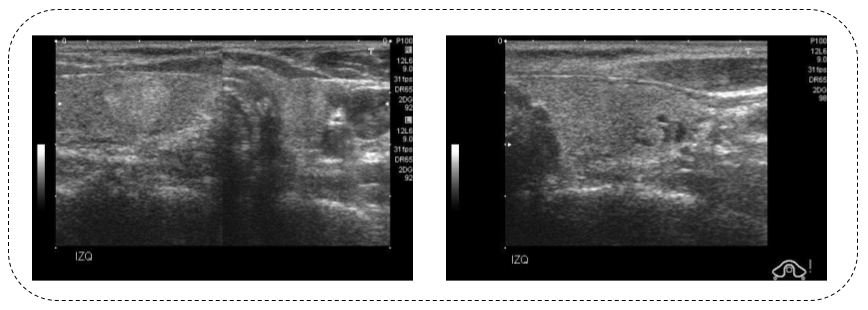
\includegraphics[width=0.85\textwidth]{4/figures/nodule_ddti.png}
		\caption[Ejemplo de imágenes del conjunto de datos de la Universidad de Colombia]{Ejemplo de imágenes del conjunto de datos de la Universidad de Colombia. \\
		Fuente: Elaboración propia.}
		\label{4:fig102}
	\end{center}
\end{figure}

\begin{figure}[H]
	\begin{center}
		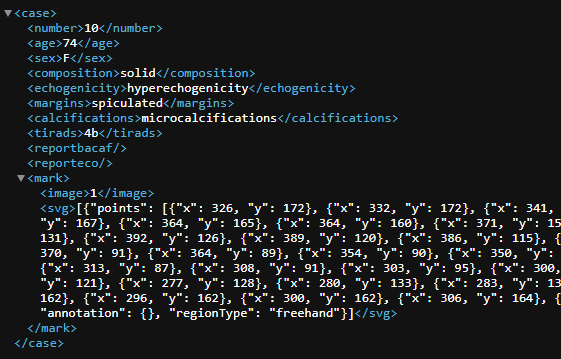
\includegraphics[width=0.65\textwidth]{4/figures/xmlfile.png}
		\caption[Ejemplo de archivo XML del conjunto de datos de la Universidad de Colombia]{Ejemplo de archivo XML del conjunto de datos de la Universidad de Colombia. \\
		Fuente: Elaboración propia.}
		\label{4:fig103}
	\end{center}
\end{figure}

Otro conjunto de datos, también de acceso libre, aunque no tan difundido como el presentado anteriormente es el otorgado por Zhujiang Hospital of Southem Medical University que recopila imágenes de 2421 pacientes obteniendo un total de 3493 imágenes de ultrasonido, de los cuales, 2283 pertenecen a imágenes de glándulas de tiroides con nódulos de carácter benigno, mientras que 1210 pertenecen a nódulos malignos. Además, este conjunto de datos también posee archivos CSV donde especifica el nombre de la imagen y la etiqueta a la que pertenece: benigno (0) o maligno (1).

Cabe destacar que este conjunto de datos posee características particulares que lo diferencian del primero, y es que este, además de estar validado por distintos comités de ética en China, procede de distintas fuentes; es decir, las imágenes pueden variar de tamaño y/o calidad entre sí.

En la Figura \ref{4:fig104} se muestran algunas imágenes de este conjunto de datos, mientras que en la Figura \ref{4:fig105} se muestra una sección de los archivos CSV.

\begin{figure}[H]
	\begin{center}
		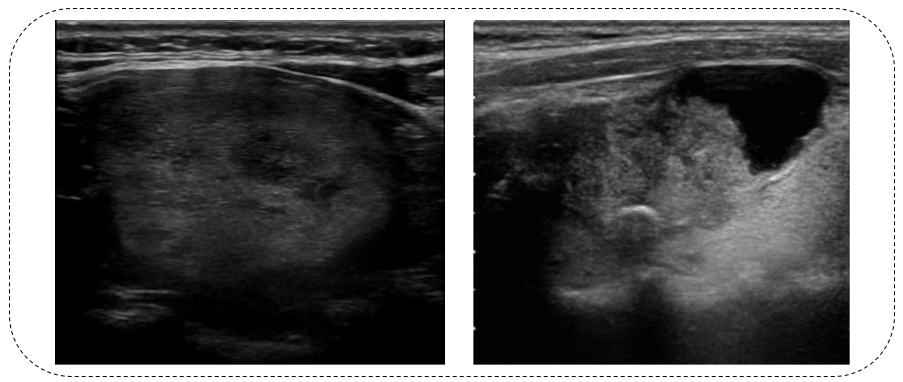
\includegraphics[width=0.68\textwidth]{4/figures/tn3k_examp.png}
		\caption[Ejemplo de imágenes del conjunto de datos de Zhujiang Hospital of Southem Medical University]{Ejemplo de imágenes del conjunto de datos de Zhujiang Hospital of Southem Medical University. \\
		Fuente: Elaboración propia.}
		\label{4:fig104}
	\end{center}
\end{figure}

\begin{figure}[H]
	\begin{center}
		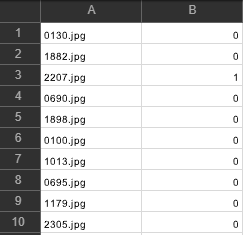
\includegraphics[width=0.38\textwidth]{4/figures/tn3k_csv.PNG}
		\caption[Ejemplo de archivo CSV del conjunto de datos de Zhujiang Hospital of Southem Medical University]{Ejemplo de archivo CSV del conjunto de datos de Zhujiang Hospital of Southem Medical University. \\
		Fuente: Elaboración propia.}
		\label{4:fig105}
	\end{center}
\end{figure}

\textbf{Actividad 2: Filtrado de los conjuntos de datos}
\\
Los requerimientos para un buen conjunto de datos radica principalmente en la información del tipo o carácter del nódulo, el origen de las imágenes de ultrasonido y la cantidad de datos.

El conjunto de datos otorgado por la Universidad de Colombia, CIM@LAB y IDIME poseía buena información, superando el requerimiento base de tipo o carácter del nódulo, pues otorgaba datos del paciente que podrían ser útiles a la hora de realizar el proceso de prediagnóstico; sin embargo, la gran debilidad del este conjunto de datos es la poca cantidad de imágenes que posee. Además, el hecho de no definirse el origen específico de estas imágenes en relación a si se obtuvo de distintas instituciones con diferentes herramientas o no, conllevó finalmente a su descarte.

El conjunto de datos de Zhujiang Hospital of Southem Medical University cumple exactamente con otorgar información sobre el carácter de los nódulos de cada imagen que posee, además, también se especifica el origen variado de las imágenes, pues fueron recopiladas de distintas instituciones y con diferentes herramientas. Finalmente, la cantidad de datos, aunque con clases desbalanceadas, supera en gran medida al primer conjunto de datos.

Al cumplir con todos los requerimientos para el entrenamiento de un buen modelo Deep Learning, el conjunto de datos finalmente seleccionado fue el de Zhujiang Hospital of Southem Medical University.

Como se mencionó en la sección anterior, la etapa siguiente es la de preprocesamiento. En este se realizó un completo análisis, limpieza y preparación de los datos para el entrenamiento de los modelos.

Cabe recordar además la existencia de dos flujos en este proceso igualmente descritos en la sección anterior. Ambos inician de igual forma con las tres siguientes actividades.

\textbf{Actividad 1: Explorar características del conjunto de datos}
\\
Ya con el conjunto de datos seleccionado, se utilizó la data almacenada en los archivos CSV (mostrado en la Figura \ref{4:fig105}) para contabilizar la cantidad de imágenes por cada clase y así determinar si existía o no la presencia de desbalance. La Figura \ref{4:fig106} y Figura \ref{4:fig107} muestran gráficas circulares donde se aprecia la proporción del total de datos por cada clase y por cada tipo de datos (entrenamiento y prueba).

\begin{figure}[H]
	\begin{center}
		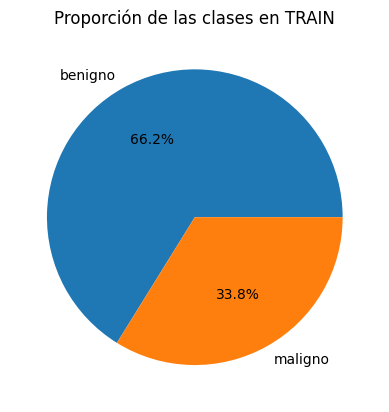
\includegraphics[width=0.51\textwidth]{4/figures/train_circular.png}
		\caption[Gráfica circular de conjunto de datos de entrenamiento]{Gráfica circular de conjunto de datos de entrenamiento. \\
		Fuente: Elaboración propia.}
		\label{4:fig106}
	\end{center}
\end{figure}

\begin{figure}[H]
	\begin{center}
		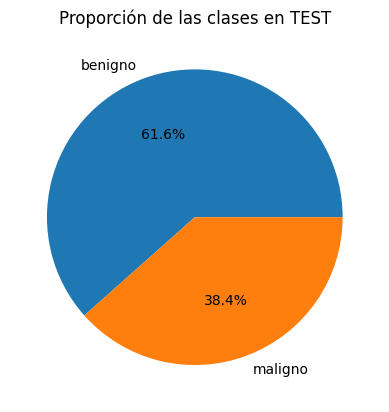
\includegraphics[width=0.51\textwidth]{4/figures/test_circular.png}
		\caption[Gráfica circular de conjunto de datos de prueba]{Gráfica circular de conjunto de datos de prueba. \\
		Fuente: Elaboración propia.}
		\label{4:fig107}
	\end{center}
\end{figure}

En ambas figuras se puede verificar la presencia de desbalance en clases, observando además como la clase de nódulos benignos duplica aproximadamente a la cantidad de imágenes de la clase de nódulos malignos. Este comportamiento se ve reflejado tanto para los datos de entrenamiento como para los de prueba.

Este descubrimiento afirmó la necesidad de aplicar una técnica de balanceo de datos.

\textbf{Actividad 2: Filtrar y organizar imágenes poco útiles del conjunto de datos}
\\
A través del Algoritmo \ref{4:alg101} se logró filtrar y obviar aquellas imágenes corruptas (en el caso de este conjunto de datos no se tuvo ninguno). Además, este también permitió la lectura de solo las imágenes con nombre presente en los archivos CSV, lo cual logró evitar el cargado de imágenes sin etiqueta alguna (en el caso de este conjunto de datos tampoco se tuvieron imágenes sin etiquetas). Finalmente, todas aquellos datos que cumplieran con los anteriores pasos serían trasladados a la nueva distribución de ficheros mostrada en la Figura \ref{4:fig109}.
%\hspace{\algorithmicindent} 
\begin{algorithm}[H]
	\caption{Proceso de organización y traslado de imágenes}
	\label{4:alg101}
	\begin{algorithmic}[1]
		\State \textbf{Entradas:} $pd\_train$, $pd\_test$, $source\_dir\_train$, $source\_dir\_test$, $train\_dir$, $test\_dir$
		\State Obtener nombres de imágenes de entrenamiento de $pd\_train$
		\State Crear diccionario $d$ de nombres a etiquetas de $pd\_train$
		\For{cada nombre de imagen $im$ en nombres de imágenes de entrenamiento}
			\State \textbf{Intentar:}
			\If{etiqueta de $im$ en $d$ es 1}
				\State Copiar $im$ a $train\_dir/malignant$
			\ElsIf{etiqueta de $im$ en $d$ es 0}
				\State Copiar $im$ a $train\_dir/benign$
			\EndIf
			\State \textbf{Excepción:}
			\State \textbf{Imprimir:} La imagen $im$ no se ha podido cargar...
		\EndFor

		\State Obtener nombres de imágenes de prueba de $pd\_test$
		\State Crear diccionario $dt$ de nombres a etiquetas de $pd\_test$
		\For{cada nombre de imagen $im$ en nombres de imágenes de prueba}
			\State \textbf{Intentar:}
			\If{etiqueta de $im$ en $dt$ es 1}
				\State Copiar $im$ a $test\_dir/malignant$
			\ElsIf{etiqueta de $im$ en $dt$ es 0}
				\State Copiar $im$ a $test\_dir/benign$
			\EndIf
			\State \textbf{Excepción:}
			\State \textbf{Imprimir:} La imagen $im$ no se ha podido cargar...
		\EndFor

		\State \textbf{Imprimir:} SE TRASLADARON TODAS LAS IMÁGENES AL NUEVO DIRECTORIO!
	\end{algorithmic}
\end{algorithm}

\begin{comment}
	\begin{figure}[H]
		\begin{center}
			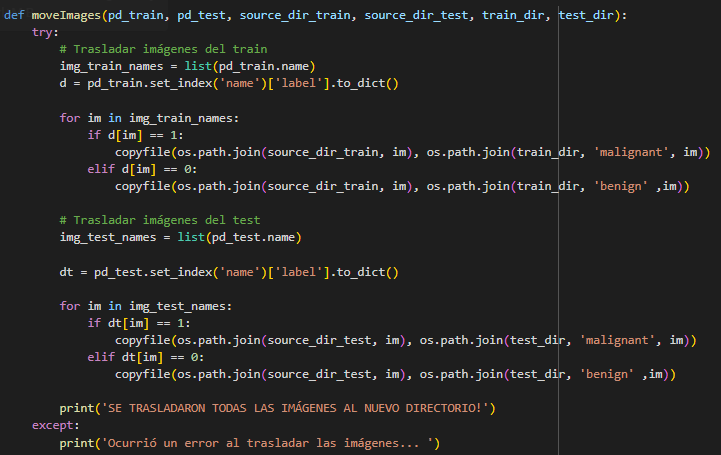
\includegraphics[width=0.75\textwidth]{4/figures/algoritm_organi.PNG}
			\caption[Algoritmo de organización de imágenes]{Algoritmo de organización de imágenes. \\
			Fuente: Elaboración propia.}
			\label{4:fig108}
		\end{center}
	\end{figure}
	
\end{comment}

\begin{figure}[H]
	\begin{center}
		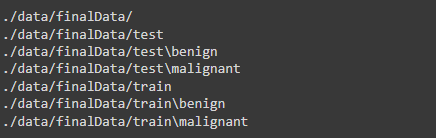
\includegraphics[width=0.60\textwidth]{4/figures/nuevos_ficheros.PNG}
		\caption[Nueva distribución de ficheros para los datos]{Nueva distribución de ficheros para los datos. \\
		Fuente: Elaboración propia.}
		\label{4:fig109}
	\end{center}
\end{figure}

\textbf{Actividad 3: Redimensionar, normalizar y dividir los datos según los requerimientos para cada modelo de Deep Learning}
\\
A partir de esta actividad, los datos usados fueron aquellos anteriormente trasladados desde los ficheros originales a los nuevos directorios.

El tamaño a redimensionar de las imágenes del conjunto de datos dependió únicamente del modelo en el que este se usó.

La normalización de los valores de píxeles de cada imagen se hizo con un media y desviación estándar de 0.5 aplicadas a cada uno de los 3 canales de las imágenes. Esto llevó a obtener finalmente píxeles con valores dentro del rango de [-1, 1], lo cual se recomienda para realizar entrenamientos de los modelos de forma más eficiente.

Finalmente, el conjunto de datos de entrenamiento se dividió en dos partes: data de validación, el cual representa el 15\% del total, y data de entrenamiento, compuesta del 85\% restante. La distribución de los datos se hizo de forma aleatoria manteniendo los mismos porcentajes.

La cantidad de la data de prueba se mantuvo igual a como originalmente fue obtenida.

Todo este proceso se realizó a través del Algoritmo \ref{4:alg102}, donde finalmente se otorgaron los tres conjuntos de datos en tipo DataLoader de Pytorch que posteriormente facilitó la ingesta de datos a los modelos.

\begin{algorithm}[H]
	\caption{Preparación de datos para entrenamiento, validación y prueba}
	\label{4:alg102}
	\begin{algorithmic}[1]
		\State \textbf{Entradas:} $train\_dir$, $test\_dir$, $img\_size$, $b\_size$
		\State \textbf{Salidas:} $train\_gen$, $val\_gen$, $test\_gen$
		
		\Procedure{DefinirTransformaciones}{}
			\State Redimensionar imágenes a $img\_size$
			\State Recortar las imágenes a $img\_size$
			\State Convertir imágenes a tensores
			\State Normalizar tensores con medias y desviaciones estándar $(0.5, 0.5, 0.5)$
		\EndProcedure
		
		\Procedure{CargarDatos}{}
			\State Cargar imágenes de entrenamiento de $train\_dir$ con transformaciones
			\State Cargar imágenes de prueba de $test\_dir$ con transformaciones
		\EndProcedure
		
		\Procedure{DividirDatosEntrenamiento}{}
			\State Calcular $val\_size$ como $15\%$ de $train\_data$
			\State Calcular $train\_size$ como $len(train\_data) - val\_size$
			\State Dividir de forma aleatoria $train\_data$ en $train\_data$ y $val\_data$ usando $train\_size$ y $val\_size$
		\EndProcedure
		
		\Procedure{CrearDataloaders}{}
			\State Crear $train\_gen$ para $train\_data$ con $b\_size$
			\State Crear $val\_gen$ para $val\_data$ con $b\_size$
			\State Crear $test\_gen$ para $test\_data$ con $b\_size$
		\EndProcedure
		
		\State \Return $train\_gen$, $val\_gen$, $test\_gen$
	\end{algorithmic}
\end{algorithm}

\begin{comment}
	\begin{figure}[H]
		\begin{center}
			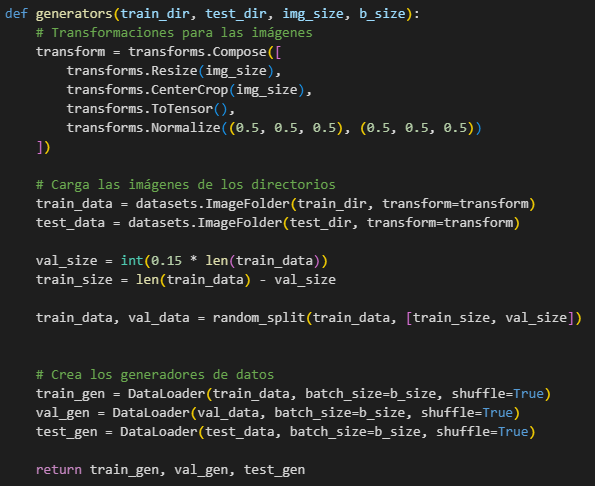
\includegraphics[width=0.70\textwidth]{4/figures/algoritm_dataloader.PNG}
			\caption[Algoritmo para lectura de los datos en DataLoader]{Algoritmo para lectura de los datos en DataLoader. \\
			Fuente: Elaboración propia.}
			\label{4:fig110}
		\end{center}
	\end{figure}
\end{comment}

\textbf{Actividad 4: Mejorar composición del conjunto de datos}
\\
Como se ha mencionado en la sección anterior de este capítulo, las características que determinan si un nódulo puede ser benigno o maligno en un imagen de ultrasonido impiden el uso de las técnicas convencionales de Aumento de Datos. Por este motivo, se construyó un modelo DCGAN con el objetivo de generar imágenes sintéticas.

Inicialmente, la arquitectura del modelo DCGAN siguió los mismos lineamientos definidos en la página oficial de Pytorch por \cite{ws_inkawhich2024dcganpytorch}; sin embargo, debido a la posible pérdida de información al reducir considerablemente el tamaño de las imágenes (ya que se pedía como entrada imágenes de 64 x 64), se decidió por personalizar el modelo original para que pueda recibir imágenes de 128 x 128, de la misma manera como se hizo en la investigación presentada por \cite{pr_JERBI2023autoclassViTGAN}. Para lograr esto se tuvo que modificar tanto la red generadora como la discriminadora.

En la red generadora se agregaron un bloque nuevo de capas similar a las que ya poseída, modificando únicamente el tamaño de canales de salida de la capa ConvTranspose2d al doble de las que poseía la capa inicial original. El tamaño de kernel, stride y padding de esta misma capa se mantuvieron del formato original. En la capa de BatchNorm2d también se duplicó la cantidad de features que recibía. La función de activación ReLU se mantuvo con la misma configuración inicial. La capas siguientes a este nuevo bloque, fueron adaptándose a la cambiada cantidad de canales de salida.

El tamaño del vector latente que ingresa a la red generadora se definió en 200, con 3 como número de canales y 128 como cantidad base de features map.

En el caso de la red discriminadora, se introdujo un bloque intermedio de capas en la parte final de todo el grupo de bloque de capas similares. La capa Conv2d de este nuevo bloque recibiría la cantidad de canales de salida del bloque anterior, mientras que sus canales de salida serían el doble de los tenía la capa Conv2d anterior. De igual forma, la capa BatchNorm2d  duplicó la cantidad de features que recibía originalmente. Se mantuvo la misma configuración de la función de activación LeakyReLU. La capa siguiente a este bloque recién creado se modificó para recibir el doble de canales de los que recibía originalmente.

La cantidad de canales que recibía el modelo se estableció en 3, mientras que el número de features map base a generar se estableció a 32.

Todas las demás configuraciones en ambas redes se dejaron por defecto.

La Figura \ref{4:fig111} muestra la arquitectura final de la red generadora.

\begin{figure}[H]
	\begin{center}
		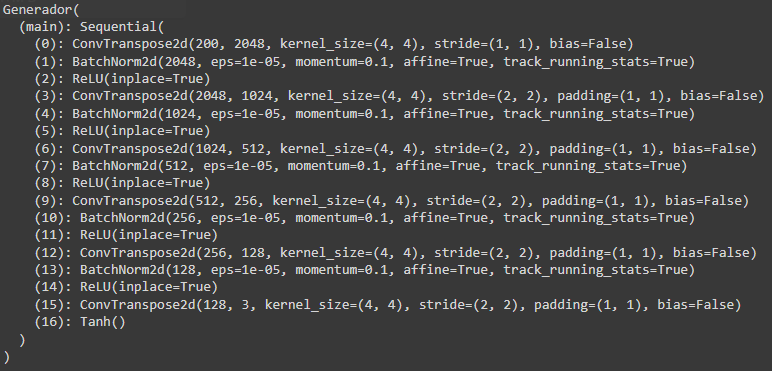
\includegraphics[width=0.78\textwidth]{4/figures/generator_network.PNG}
		\caption[Arquitectura de Red Generadora]{Arquitectura de Red Generadora. \\
		Fuente: Elaboración propia.}
		\label{4:fig111}
	\end{center}
\end{figure}

De igual forma, la Figura \ref{4:fig112}, muestra la arquitectura de la red discriminadora. 

\begin{figure}[H]
	\begin{center}
		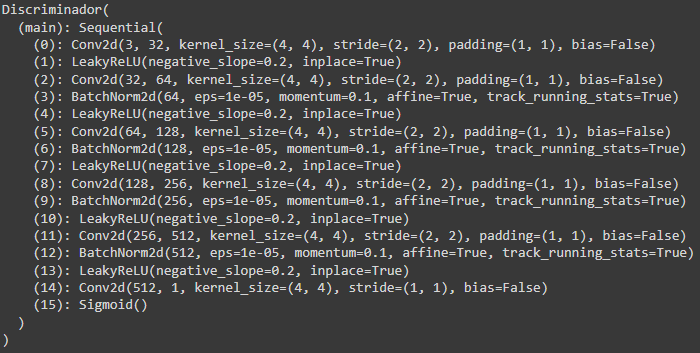
\includegraphics[width=0.76\textwidth]{4/figures/discriminator_network.PNG}
		\caption[Arquitectura de Red Discriminadora]{Arquitectura de Red Discriminadora. \\
		Fuente: Elaboración propia.}
		\label{4:fig112}
	\end{center}
\end{figure}

Para la función de pérdida se usó el Binary Cross Entropy Loss, mientras que la función de optimización se estableció en Adam con una tasa de aprendizaje de 0.0002 y betas de 0.5 para el primero y 0.999 para el segundo. Todo esto según lo establecido por la página oficial de Pytorch.

También se definió un tensor fijo de tamaño 200 (tamaño anteriormente definido de vector latente) inicializado con números aleatorios pero que siguen una distribución normal. Este tensor tenía un lote de tamaño 64.

Para ya iniciar con el entrenamiento del modelo DCGAN se procedió con la creación del DataLoader de Pytorch que contenía todas las imágenes del conjunto de datos de entrenamiento. En este proceso, se definió que las imágenes deberían ser redimensionadas a tamaño 128 y con leídas en un tamaño de lote 64.

El proceso de entrenamiento siguió las características normales del DCGAN original, estableciendo únicamente la cantidad de épocas a 200.

Se usó las capacidades de la GPU NVIDIA A100-SXM4-40GB obtenido a través de Google Colab para este proceso de entrenamiento.

En la Figura \ref{4:fig113} se muestran las métricas de la parte final del entrenamiento.

\begin{figure}[H]
	\begin{center}
		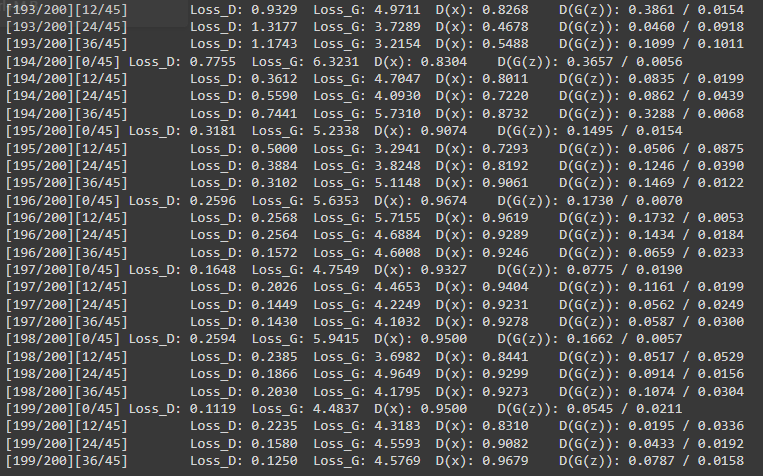
\includegraphics[width=0.75\textwidth]{4/figures/dcgan_1_train.PNG}
		\caption[Parte final del entrenamietno del DCGAN]{Parte final del entrenamietno del DCGAN. \\
		Fuente: Elaboración propia.}
		\label{4:fig113}
	\end{center}
\end{figure}

Además, se realizó un plot de las pérdidas de ambas redes a través de cada iteración del entrenamiento del modelo. Este se muestra en la Figura \ref{4:fig114}.

\begin{figure}[H]
	\begin{center}
		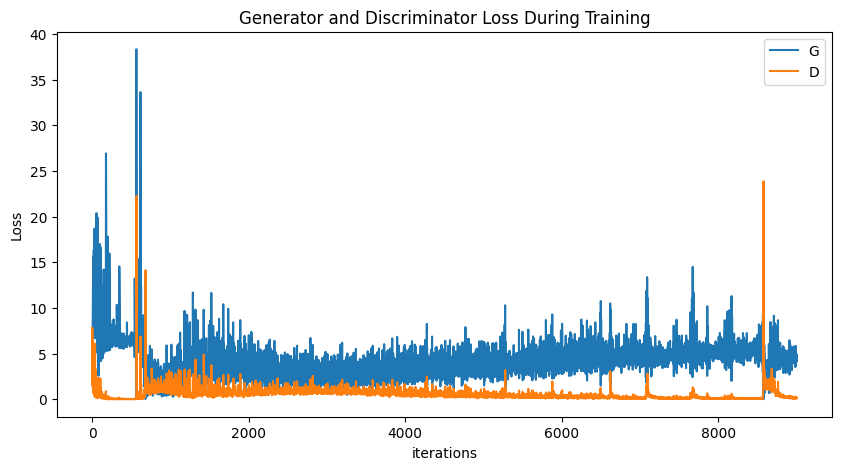
\includegraphics[width=0.85\textwidth]{4/figures/plot_loss_1.png}
		\caption[Plot de pérdidas de las red Generadora y Discriminadora]{Plot de pérdidas de las red Generadora y Discriminadora. \\
		Fuente: Elaboración propia.}
		\label{4:fig114}
	\end{center}
\end{figure}

En esta última gráfica se puede observar cómo ambas pérdidas van convergiendo a más iteraciones se tiene; sin embargo, ya en la parte final se logra observar la divergencia de ambos valores. Esto podría deberse a un sobreajuste por parte de la red discriminadora, al mismo tiempo que la red generadora deja de mejorar en la tarea de generar imágenes sintéticas.

Las imágenes reales y generadas se muestran en la Figura \ref{4:fig115}.

\begin{figure}[H]
	\begin{center}
		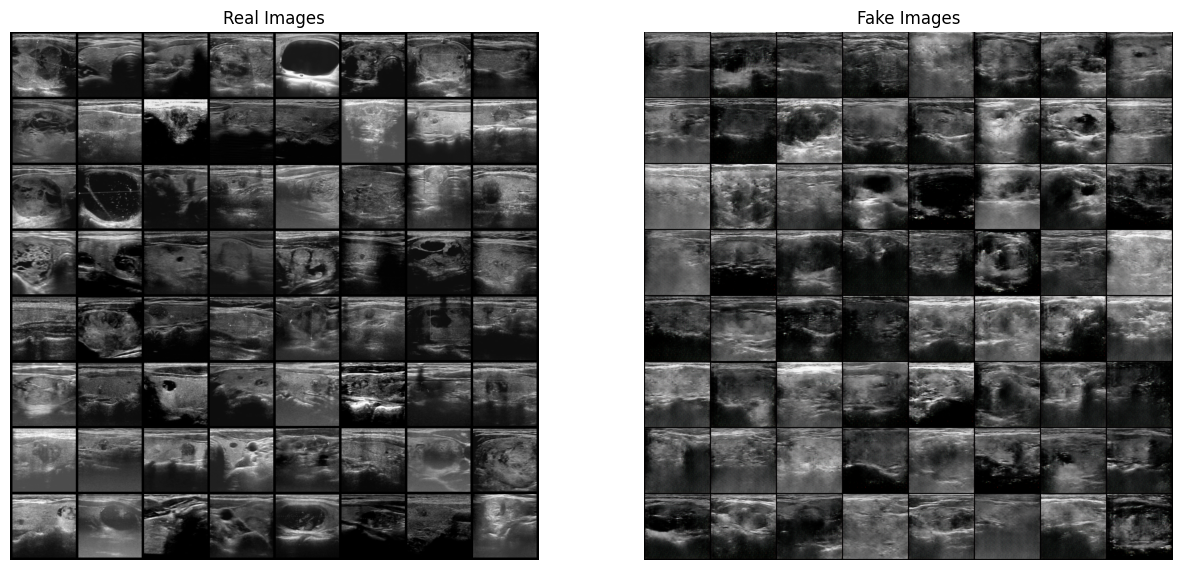
\includegraphics[width=0.85\textwidth]{4/figures/generated_real_1.png}
		\caption[Imágenes de ultrasonido de nódulos tiroideos generados y reales]{Imágenes de ultrasonido de nódulos tiroideos generados y reales. \\
		Fuente: Elaboración propia.}
		\label{4:fig115}
	\end{center}
\end{figure}

Según un rápido análisis visual, la imágenes generadas sí tienen un poco de similitud a las originales, y fácilmente, para alguien no experto, estos podrían pasar como imágenes reales.

Ya que el entrenamiento se realizó con todas las imágenes la data de entrenamiento, todas las imágenes generadas podrían pertenecer a cualquiera de las clases (benigno o maligno) y se es difícil sino imposible determinar a qué tipo pertenecen (benigno o maligno). Por este motivo, y viendo el potencial del DCGAN, se volvió a entrenar el modelo ahora solo con imágenes de la clase maligno (clase minoritaria) del conjunto de datos de entrenamiento para que la red solo pueda generar imágenes de ultrasonido de esta clase en específico.

En este caso se modificó el tamaño de vector latente a 300 y los features map base a 256 en la red generadora. Las demás configuraciones se mantuvieron, incluyendo aquellas de la red discriminadora.

Se usaron la misma función de pérdida y optimización con los mismos parámetros definidos anteriormente.

El tensor fijo de números aleatorio de distribución normal tuvo para este entrenamiento un tamaño de 300 (igual al tamaño del vector latente).

Para el DataLoader se mantuvo el mismo tamaño de redimensionamiento y lote.

Debido a una prueba rápida inicial con una menor cantidad de épocas, donde se obtuvieron pobres resultados, se decidió aumentar la cantidad de iteraciones totales estableciendo el número de épocas a 370.

La Figura \ref{4:fig116} muestra la parte final del entrenamiento.

\begin{figure}[H]
	\begin{center}
		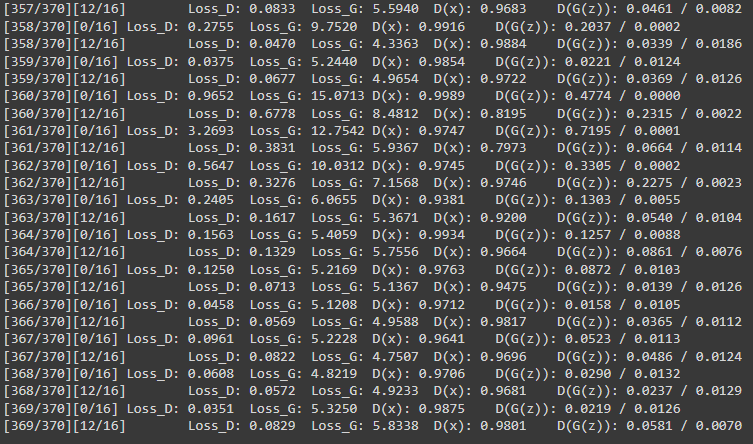
\includegraphics[width=0.75\textwidth]{4/figures/dcgan_2_train.PNG}
		\caption[Parte final del entrenamietno del DCGAN con imágenes de nódulos malignos]{Parte final del entrenamietno del DCGAN con imágenes de nódulos malignos. \\
		Fuente: Elaboración propia.}
		\label{4:fig116}
	\end{center}
\end{figure}

De igual manera al entrenamiento inicial, se realizó una gráfica donde se muestra el comportamiento de la pérdida en ambas redes. Esto se muestra en la Figura \ref{4:fig117}.

\begin{figure}[H]
	\begin{center}
		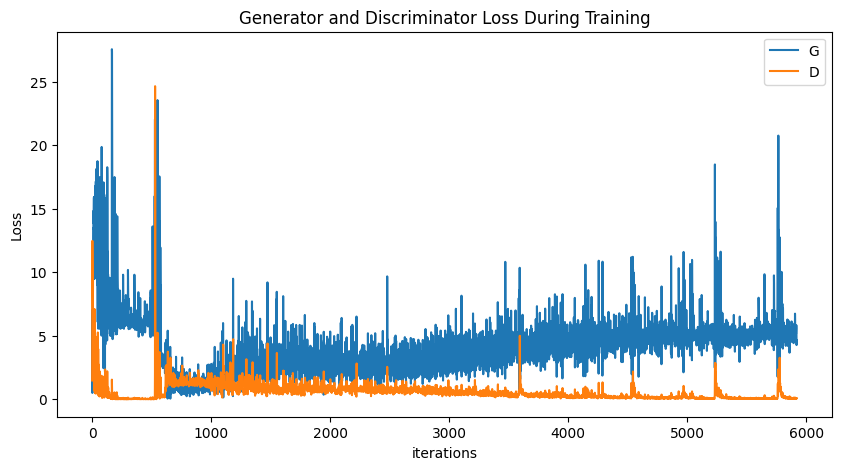
\includegraphics[width=0.85\textwidth]{4/figures/plot_loss_2.png}
		\caption[Plot de pérdidas de las red Generadora y Discriminadora de imágenes de nódulos malignos]{Plot de pérdidas de las red Generadora y Discriminadora de imágenes de nódulos malignos. \\
		Fuente: Elaboración propia.}
		\label{4:fig117}
	\end{center}
\end{figure}

Esta gráfica muestra el mismo comportamiento que a más iteraciones, mayor divergencia entre las pérdidas.

En la Figura \ref{4:fig118} se presentan las imágenes generadas junto a las originales.

\begin{figure}[H]
	\begin{center}
		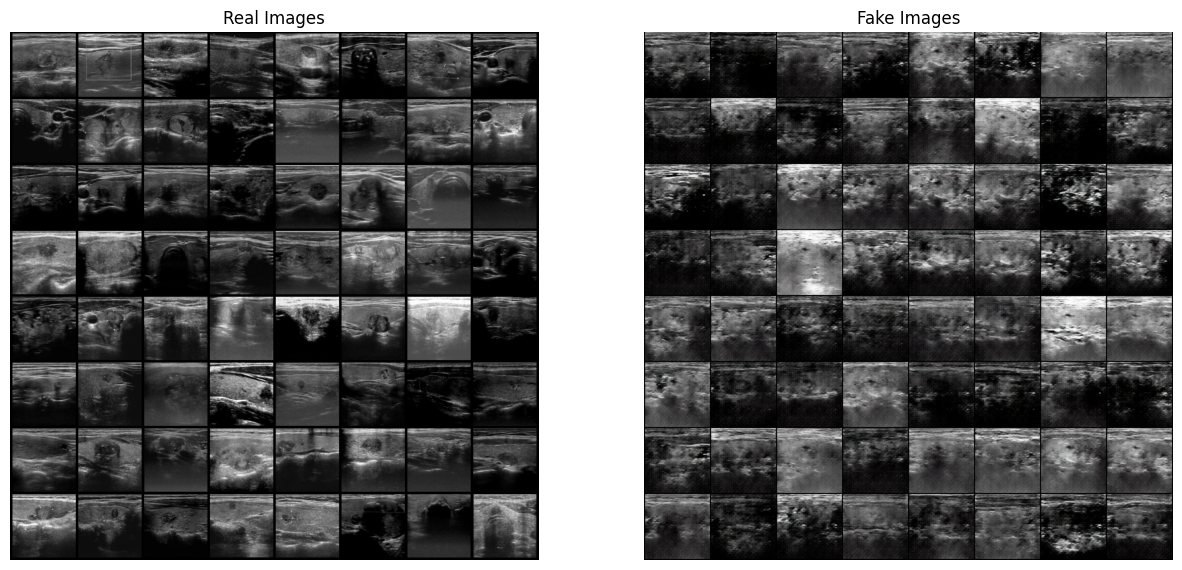
\includegraphics[width=0.85\textwidth]{4/figures/generated_real_2.png}
		\caption[Imágenes de ultrasonido de nódulos tiroideos generados y reales (DCGAN de imágenes de nódulos malignos)]{Imágenes de ultrasonido de nódulos tiroideos generados y reales (DCGAN de imágenes de nódulos malignos). \\
		Fuente: Elaboración propia.}
		\label{4:fig118}
	\end{center}
\end{figure}

Los resultados de las imágenes generadas en este modelo muestran mayor ruido comparado las generadas con el entrenamiento inicial, esto se debe principalmente a la menor cantidad de datos usada para el entrenamiento de este nuevo DCGAN. Sin embargo, luego de un rápido análisis visual, se puede observar un comportamiento similar entre todas estas imágenes nuevas, y es que en la mayoría de estas hay lo que parece ser la presencia de un nódulo, aunque difuminado con mucho ruido aleatorio, esto podría indicar un aprendizaje cercano a la distribución de las imágenes de nódulos malignos.

Intentando utilizar el potencial que ofrece el DCGAN, se realizó posteriormente dos tipos de entrenamiento a los modelos de Deep Learning: el primero sin el Aumento de Datos a través de DCGAN, mientras que el segundo combinará los datos generados con la data original de entrenamiento para realizar dicho proceso. Esto permitirá determinar si las imágenes generadas por el DCGAN, aunque con ruido, son capaces de aumentar la capacidad de predicción de los modelos.

La gráfica circula presenta en la Figura \ref{4:fig119} muestra el nuevo balance entre ambas clases en la nueva data de entrenamiento.

\begin{figure}[H]
	\begin{center}
		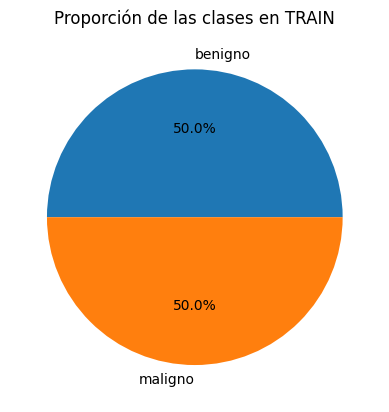
\includegraphics[width=0.51\textwidth]{4/figures/balanced_circular.png}
		\caption[Gráfica circula de data de entrenamiento balanceada]{Gráfica circula de data de entrenamiento balanceada. \\
		Fuente: Elaboración propia.}
		\label{4:fig119}
	\end{center}
\end{figure}

Ya con la data preprocesada, se inició con la etapa de Aplicación de Deep Learning donde se entrenó, validó y puso a prueba los diversos modelos CNN y ViT. Esta etapa inicia con la siguiente actividad.

\textbf{Actividad 1: Seleccionar algoritmos a entrenar según usos y resultados de las investigaciones presentadas en los antecedentes}
\\
Según los datos analizados en las investigaciones presentadas en el Capítulo 2, el modelo con mayor presencia de los CNN es el ResNet50, mientras que por el lado de los modelos ViT, los más usados son los ViT-Base con tamaño de patch de 16 x 16.

Además, debido al tipo de problema de clasificación presente en esta investigación, y la similitud con el trabajo de \cite{pr_JERBI2023autoclassViTGAN}, se decidió por probar con las redes VGG16, ya que ha demostrado ser capaz de obtener un alto desempeño.

En resumen, se ha optado por utilizar las arquitecturas CNN de ResNet50 y VGG16. Además, como parte de las arquitecturas ViT, se optó por el uso de ViT-Base (16).

\textbf{Actividad 2: Entrenar y probar los modelos de Deep Learning previamente definidos}
\\
Para todas las arquitecturas de Deep Learning en esta investigación, se definió como función de activación el sigmoide. De igual manera, para el entrenamiento se usó la capacidad de la GPU NVIDIA A100-SXM4-40GB obtenido a través de Google Colab para lograr un rápido y eficiente entrenamiento. Además, se determinó una semilla de 2024 para permitir la reproducibilidad de los resultados. 

En este primer grupo, no se utilizará el conjunto de datos con imágenes generadas.

Se empezó con los modelos ViT-Base (16).

Para este proceso se crearon los DataLoader correspondientes con las características requeridas por estos modelos ViT: se redimensionaron las imágenes a 224 x 224 y se definió un tamaño de lote de 64 (este último tamaño será constante para todos los modelos mostrados en esta actividad).

En este primer modelo, se usó la técnica de entrenamiento de Fine Tuning junto con el modelo ViT-Base (16) con pesos de IMAGENET1KV1.

La función de pérdida aplicada fue el BCEWithLogitsLoss que evita el uso manual de la sigmoide y lo aplica directamente con la entropía cruzada. Nuevamente, esta función será utilizada en cada uno de los modelos en esta actividad.

Para lograr una clasificación binaria, las últimas capas de estas arquitecturas debió ser reemplazada por un MLP simple que recibe todos los features del modelo y produce una única salida. La configuración del MLP se definió de la forma (256, 1), donde el primer valor es el número de neuronas en la capas oculta que tuvo la función de activación ReLU, y el segundo valor es el número de neuronas en la capa de salida. Esta configuración de MLP se aplicó a todos los modelos ViT y CNN, a excepción de VGG16, donde se usó una configuración por defecto, únicamente modificando a 1 el número de neuronas en la capa de salida. En el caso de los modelos híbridos, solamente se etableció el bloque clasificador a una capa de salida con 1 neurona, debido a las limitaciones de disponibilidad de recursos computacionales.

Finalmente, la función de optimización utilizada fue Adam con una tasa de aprendizaje de 0.0001, y se definió para el entrenamiento 20 épocas. Las demás configuraciones se dejaron por defecto.

Estas configuraciones se aplicarán de igual manera a los demás modelos en esta actividad.

A continuación se presenta en la Figura \ref{4:fig120} el proceso de entrenamiento del modelo ViT-Base (16) con los pesos IMAGENET1KV1 y usando la técnica de Fine Tuning.

\begin{figure}[H]
	\begin{center}
		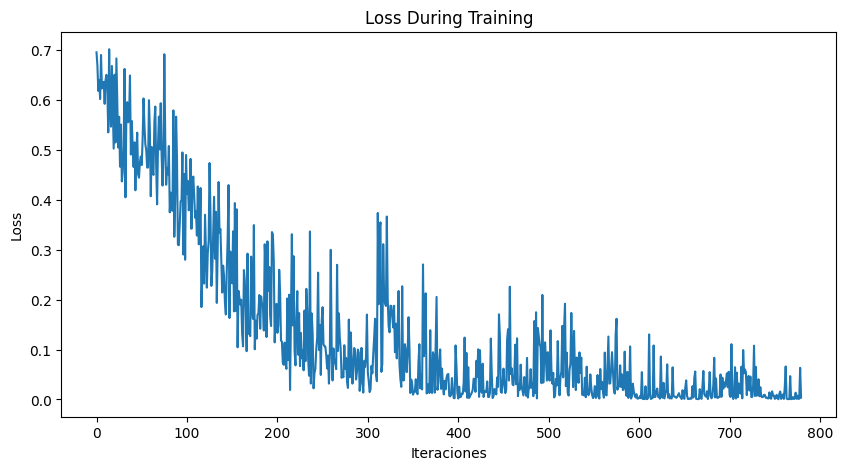
\includegraphics[width=0.85\textwidth]{4/figures/model1_train.PNG}
		\caption[Proceso de entrenamiento del modelo n°1]{Proceso de entrenamiento del modelo n°1. \\
		Fuente: Elaboración propia.}
		\label{4:fig120}
	\end{center}
\end{figure}

Finalmente, para este modelo también se calcularon su Accuracy, Recall y Precision. Estos son presentados en la Tabla \ref{4:table2}.

\begin{table}[H]
	\caption[Accuracy, Recall y Precision del modelo n°1]{Accuracy, Recall y Precision del modelo n°1.}
	\label{4:table2}
	\centering
	\small
	\begin{tabular}{c|ccc}
		\specialrule{.1em}{.05em}{.05em}
		{Métrica} & {Accuracy} & {Recall} & {Precision} \\
		\hline
		{Valor} & {69.54\%} & {47.03\%} & {64.16\%} \\
		\specialrule{.1em}{.05em}{.05em}
	\end{tabular}
	\begin{flushleft}	
		\small Fuente: Elaboración propia.
	\end{flushleft}
\end{table}

\begin{comment}
\begin{figure}[H]
	\begin{center}
		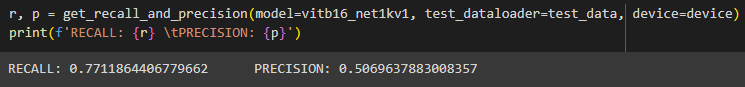
\includegraphics[width=0.83\textwidth]{4/figures/model1_rp.PNG}
		\caption[Accuracy, Recall y Precision del modelo n°1]{Recall y Precision del modelo n°1. \\
		Fuente: Elaboración propia.}
		\label{4:fig121}
	\end{center}
\end{figure}
\end{comment}

En el siguiente modelo, se usó la técnica de entrenamiento de Transfer Learning junto con el modelo ViT-Base (16) con pesos de IMAGENET1KV1.

El DataLoader constaba de las imágenes redimensionadas nuevamente a 224 x 224, y se aplicó la función de pérdida BCEWithLogitsLoss junto con la función de optimización Adam.

A continuación se presenta en la Figura \ref{4:fig122} el proceso de entrenamiento del modelo ViT-Base (16) con los pesos IMAGENET1KV1 y usando la técnica de Transfer Learning.

\begin{figure}[H]
	\begin{center}
		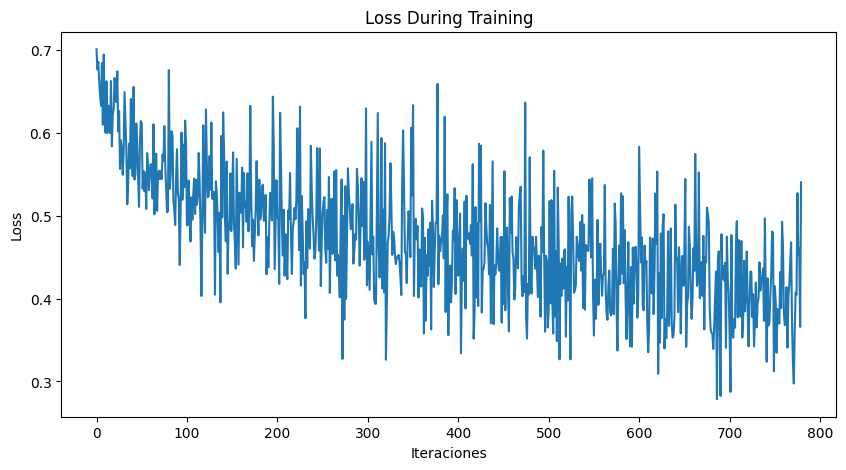
\includegraphics[width=0.85\textwidth]{4/figures/model2_train.PNG}
		\caption[Proceso de entrenamiento del modelo n°2]{Proceso de entrenamiento del modelo n°2. \\
		Fuente: Elaboración propia.}
		\label{4:fig122}
	\end{center}
\end{figure}

También se calcularon su Accuracy, Recall y Precision. Estos son presentados en la Tabla \ref{4:table3}.

\begin{table}[H]
	\caption[Accuracy, Recall y Precision del modelo n°2]{Accuracy, Recall y Precision del modelo n°2.}
	\label{4:table3}
	\centering
	\small
	\begin{tabular}{c|ccc}
		\specialrule{.1em}{.05em}{.05em}
		{Métrica} & {Accuracy} & {Recall} & {Precision} \\
		\hline
		{Valor} & {68.08\%} & {53.39\%} & {59.43\%} \\
		\specialrule{.1em}{.05em}{.05em}
	\end{tabular}
	\begin{flushleft}	
		\small Fuente: Elaboración propia.
	\end{flushleft}
\end{table}

\begin{comment}
\begin{figure}[H]
	\begin{center}
		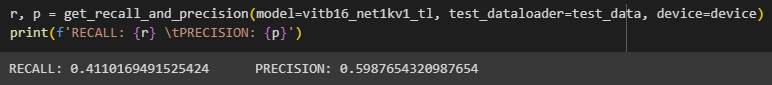
\includegraphics[width=0.83\textwidth]{4/figures/model2_rp.PNG}
		\caption[Recall y Precision del modelo n°2]{Recall y Precision del modelo n°2. \\
		Fuente: Elaboración propia.}
		\label{4:fig123}
	\end{center}
\end{figure}
\end{comment}

Este modelo usó la técnica de entrenamiento de Fine Tuning junto con el modelo ViT-Base (16) con pesos de IMAGENET1KSWAGE2EV1.

En este caso, el DataLoader constaba de las imágenes redimensionadas a 384 x 384.

Se presenta en la Figura \ref{4:fig124} el proceso de entrenamiento del modelo ViT-Base (16) con los pesos  IMAGENET1KSWAGE2EV1 y usando la técnica de Fine Tuning.

\begin{figure}[H]
	\begin{center}
		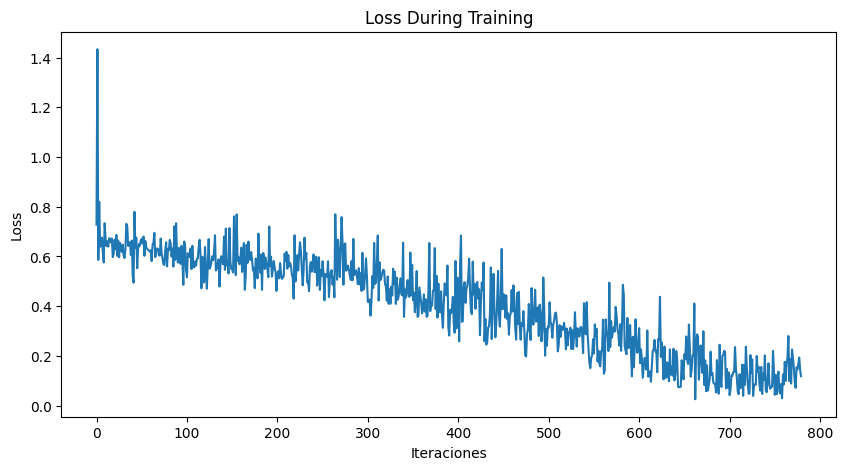
\includegraphics[width=0.85\textwidth]{4/figures/model3_train.PNG}
		\caption[Proceso de entrenamiento del modelo n°3]{Proceso de entrenamiento del modelo n°3. \\
		Fuente: Elaboración propia.}
		\label{4:fig124}
	\end{center}
\end{figure}

También se calcularon su Accuracy, Recall y Precision. Estos son presentados en la Tabla \ref{4:table4}.

\begin{table}[H]
	\caption[Accuracy, Recall y Precision del modelo n°3]{Accuracy, Recall y Precision del modelo n°3.}
	\label{4:table4}
	\centering
	\small
	\begin{tabular}{c|ccc}
		\specialrule{.1em}{.05em}{.05em}
		{Métrica} & {Accuracy} & {Recall} & {Precision} \\
		\hline
		{Valor} & {56.84\%} & {53.81\%} & {44.88\%} \\
		\specialrule{.1em}{.05em}{.05em}
	\end{tabular}
	\begin{flushleft}	
		\small Fuente: Elaboración propia.
	\end{flushleft}
\end{table}

\begin{comment}
\begin{figure}[H]
	\begin{center}
		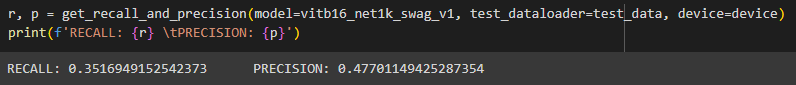
\includegraphics[width=0.83\textwidth]{4/figures/model3_rp.PNG}
		\caption[Recall y Precision del modelo n°3]{Recall y Precision del modelo n°3. \\
		Fuente: Elaboración propia.}
		\label{4:fig125}
	\end{center}
\end{figure}
\end{comment}

El modelo n°4 empleó la técnica de entrenamiento de Transfer Learning junto con el modelo ViT-Base (16) con pesos de IMAGENET1KSWAGE2EV1.

En este caso, nuevamente el DataLoader constaba de las imágenes redimensionadas a 384 x 384.

Se presenta en la Figura \ref{4:fig126} el proceso de entrenamiento del modelo ViT-Base (16) con los pesos IMAGENET1KSWAGE2EV1 y usando la técnica de Transfer Learning.

\begin{figure}[H]
	\begin{center}
		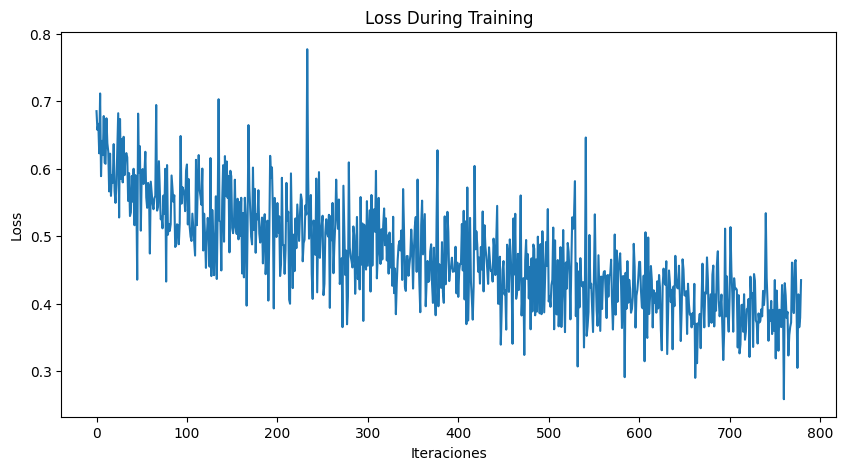
\includegraphics[width=0.85\textwidth]{4/figures/model4_train.PNG}
		\caption[Proceso de entrenamiento del modelo n°4]{Proceso de entrenamiento del modelo n°4. \\
		Fuente: Elaboración propia.}
		\label{4:fig126}
	\end{center}
\end{figure}

También se calcularon su Accuracy, Recall y Precision. Estos son presentados en la Tabla \ref{4:table5}.

\begin{table}[H]
	\caption[Accuracy, Recall y Precision del modelo n°4]{Accuracy, Recall y Precision del modelo n°4.}
	\label{4:table5}
	\centering
	\small
	\begin{tabular}{c|ccc}
		\specialrule{.1em}{.05em}{.05em}
		{Métrica} & {Accuracy} & {Recall} & {Precision} \\
		\hline
		{Valor} & {69.22\%} & {55.51\%} & {60.93\%} \\
		\specialrule{.1em}{.05em}{.05em}
	\end{tabular}
	\begin{flushleft}	
		\small Fuente: Elaboración propia.
	\end{flushleft}
\end{table}

\begin{comment}
\begin{figure}[H]
	\begin{center}
		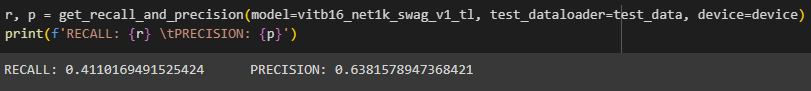
\includegraphics[width=0.83\textwidth]{4/figures/model4_rp.PNG}
		\caption[Recall y Precision del modelo n°4]{Recall y Precision del modelo n°4. \\
		Fuente: Elaboración propia.}
		\label{4:fig127}
	\end{center}
\end{figure}
\end{comment}

El modelo n°5 empleó la técnica de entrenamiento de Fine Tuning junto con el modelo ViT-Base (16) con pesos de IMAGENET1KSWAGLINEARV1.

En este caso, el DataLoader constaba de las imágenes redimensionadas a 224 x 224.

Se presenta en la Figura \ref{4:fig128} el proceso de entrenamiento del modelo ViT-Base (16) con los pesos IMAGENET1KSWAGLINEARV1 y usando la técnica de Fine Tuning.

\begin{figure}[H]
	\begin{center}
		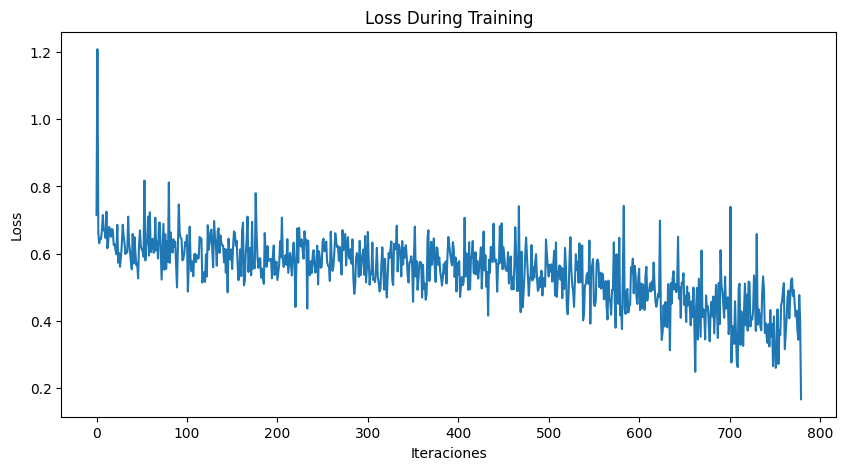
\includegraphics[width=0.85\textwidth]{4/figures/model5_train.PNG}
		\caption[Proceso de entrenamiento del modelo n°5]{Proceso de entrenamiento del modelo n°5. \\
		Fuente: Elaboración propia.}
		\label{4:fig128}
	\end{center}
\end{figure}

También se calcularon su Recall y Precision. Estos son presentados en la Tabla \ref{4:table6}.

\begin{table}[H]
	\caption[Accuracy, Recall y Precision del modelo n°5]{Accuracy, Recall y Precision del modelo n°5.}
	\label{4:table6}
	\centering
	\small
	\begin{tabular}{c|ccc}
		\specialrule{.1em}{.05em}{.05em}
		{Métrica} & {Accuracy} & {Recall} & {Precision} \\
		\hline
		{Valor} & {58.47\%} & {34.75\%} & {44.81\%} \\
		\specialrule{.1em}{.05em}{.05em}
	\end{tabular}
	\begin{flushleft}	
		\small Fuente: Elaboración propia.
	\end{flushleft}
\end{table}

\begin{comment}
\begin{figure}[H]
	\begin{center}
		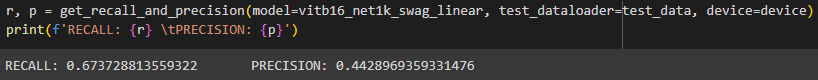
\includegraphics[width=0.83\textwidth]{4/figures/model5_rp.PNG}
		\caption[Recall y Precision del modelo n°5]{Recall y Precision del modelo n°5. \\
		Fuente: Elaboración propia.}
		\label{4:fig129}
	\end{center}
\end{figure}
\end{comment}

El modelo n°6 empleó la técnica de entrenamiento de Transfer Learning junto con el modelo ViT-Base (16) con pesos de IMAGENET1KSWAGLINEARV1.

En este caso, el DataLoader constaba nuevamente de las imágenes redimensionadas a 224 x 224.

Se presenta en la Figura \ref{4:fig130} el proceso de entrenamiento del modelo ViT-Base (16) con los pesos IMAGENET1KSWAGLINEARV1 y usando la técnica de Transfer Learning.

\begin{figure}[H]
	\begin{center}
		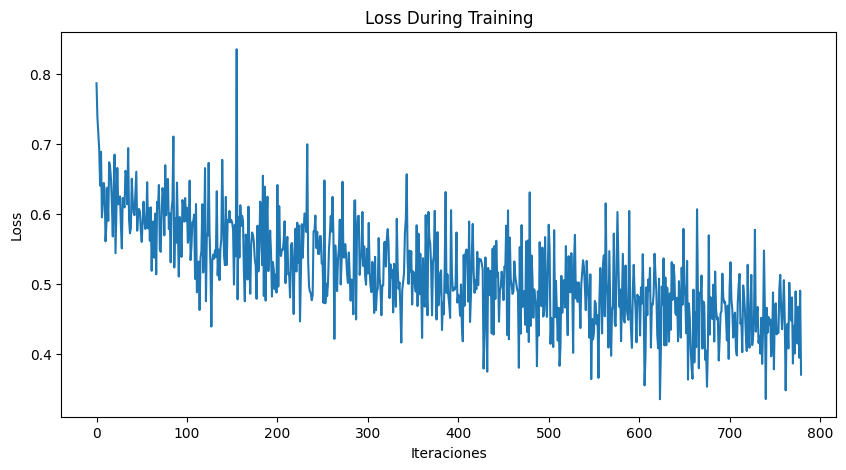
\includegraphics[width=0.85\textwidth]{4/figures/model6_train.PNG}
		\caption[Proceso de entrenamiento del modelo n°6]{Proceso de entrenamiento del modelo n°6. \\
		Fuente: Elaboración propia.}
		\label{4:fig130}
	\end{center}
\end{figure}

También se calcularon su Accuracy, Recall y Precision. Estos son presentados en la Tabla \ref{4:table7}.

\begin{table}[H]
	\caption[Accuracy, Recall y Precision del modelo n°6]{Accuracy, Recall y Precision del modelo n°6.}
	\label{4:table7}
	\centering
	\small
	\begin{tabular}{c|ccc}
		\specialrule{.1em}{.05em}{.05em}
		{Métrica} & {Accuracy} & {Recall} & {Precision} \\
		\hline
		{Valor} & {65.31\%} & {41.95\%} & {56.57\%} \\
		\specialrule{.1em}{.05em}{.05em}
	\end{tabular}
	\begin{flushleft}	
		\small Fuente: Elaboración propia.
	\end{flushleft}
\end{table}

\begin{comment}
\begin{figure}[H]
	\begin{center}
		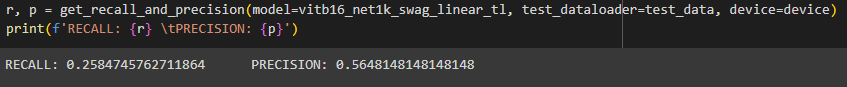
\includegraphics[width=0.83\textwidth]{4/figures/model6_rp.PNG}
		\caption[Recall y Precision del modelo n°6]{Recall y Precision del modelo n°6. \\
		Fuente: Elaboración propia.}
		\label{4:fig131}
	\end{center}
\end{figure}
\end{comment}

El modelo n°7 empleó la técnica de entrenamiento de Fine Tuning junto con el modelo VGG16 con pesos de IMAGENET1KV1.

En este caso, el DataLoader fue cargado con imágenes redimensionadas a 128 x 128. Este tamaño será constante para los demás modelos CNN.

Se presenta en la Figura \ref{4:fig132} el proceso de entrenamiento del modelo VGG16 con los pesos IMAGENET1KV1 y usando la técnica de Fine Tuning.

\begin{figure}[H]
	\begin{center}
		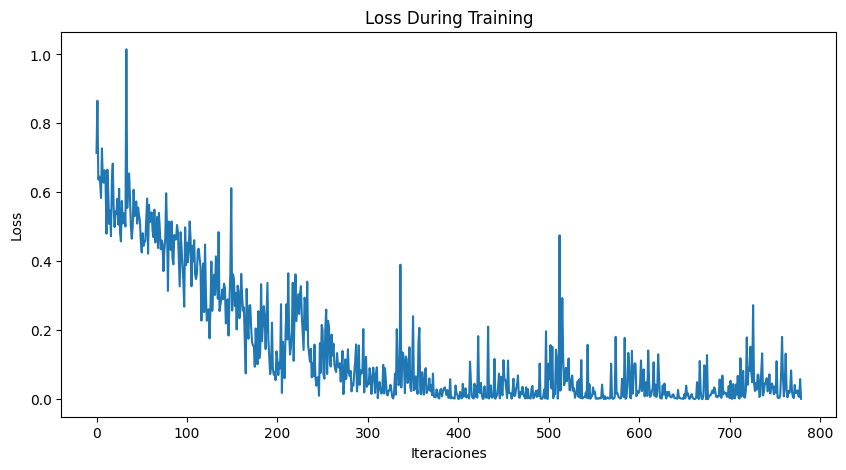
\includegraphics[width=0.85\textwidth]{4/figures/model7_train.PNG}
		\caption[Proceso de entrenamiento del modelo n°7]{Proceso de entrenamiento del modelo n°7. \\
		Fuente: Elaboración propia.}
		\label{4:fig132}
	\end{center}
\end{figure}

También se calcularon su Accuracy, Recall y Precision. Estos son presentados en la Tabla \ref{4:table8}.

\begin{table}[H]
	\caption[Accuracy, Recall y Precision del modelo n°7]{Accuracy, Recall y Precision del modelo n°7.}
	\label{4:table8}
	\centering
	\small
	\begin{tabular}{c|ccc}
		\specialrule{.1em}{.05em}{.05em}
		{Métrica} & {Accuracy} & {Recall} & {Precision} \\
		\hline
		{Valor} & {71.99\%} & {58.90\%} & {64.95\%} \\
		\specialrule{.1em}{.05em}{.05em}
	\end{tabular}
	\begin{flushleft}	
		\small Fuente: Elaboración propia.
	\end{flushleft}
\end{table}

\begin{comment}
\begin{figure}[H]
	\begin{center}
		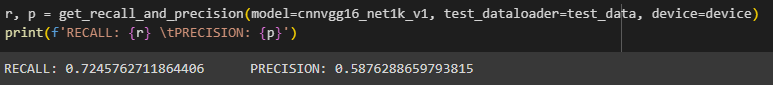
\includegraphics[width=0.83\textwidth]{4/figures/model7_rp.PNG}
		\caption[Recall y Precision del modelo n°7]{Recall y Precision del modelo n°7. \\
		Fuente: Elaboración propia.}
		\label{4:fig133}
	\end{center}
\end{figure}
\end{comment}

El modelo n°8 empleó la técnica de entrenamiento de Transfer Learning junto con el modelo VGG16 con pesos de IMAGENET1KV1.

Se presenta en la Figura \ref{4:fig134} el proceso del entrenamiento del modelo VGG16 con los pesos IMAGENET1KV1 y usando la técnica de Transfer Learning.

\begin{figure}[H]
	\begin{center}
		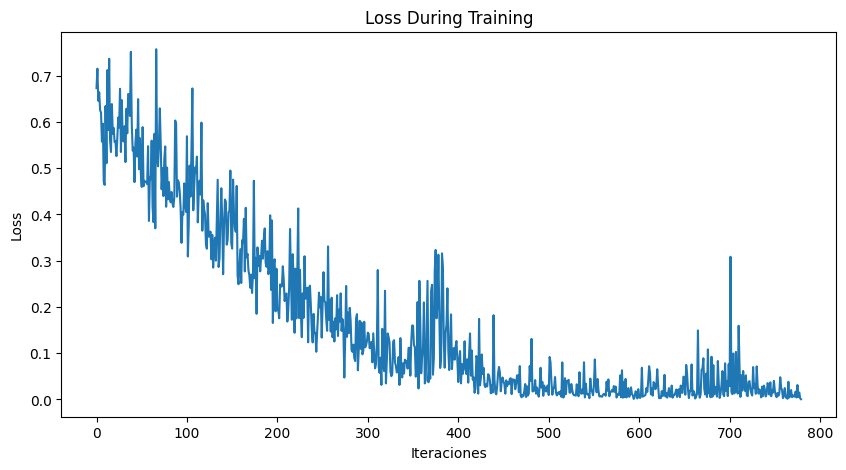
\includegraphics[width=0.85\textwidth]{4/figures/model8_train.PNG}
		\caption[Proceso de entrenamiento del modelo n°8]{Proceso de entrenamiento del modelo n°8. \\
		Fuente: Elaboración propia.}
		\label{4:fig134}
	\end{center}
\end{figure}

También se calcularon su Accuracy, Recall y Precision. Estos son presentados en la Tabla \ref{4:table9}.

\begin{table}[H]
	\caption[Accuracy, Recall y Precision del modelo n°8]{Accuracy, Recall y Precision del modelo n°8.}
	\label{4:table9}
	\centering
	\small
	\begin{tabular}{c|ccc}
		\specialrule{.1em}{.05em}{.05em}
		{Métrica} & {Accuracy} & {Recall} & {Precision} \\
		\hline
		{Valor} & {65.80\%} & {67.37\%} & {54.45\%} \\
		\specialrule{.1em}{.05em}{.05em}
	\end{tabular}
	\begin{flushleft}	
		\small Fuente: Elaboración propia.
	\end{flushleft}
\end{table}

\begin{comment}
\begin{figure}[H]
	\begin{center}
		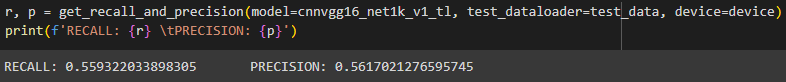
\includegraphics[width=0.83\textwidth]{4/figures/model8_rp.PNG}
		\caption[Recall y Precision del modelo n°8]{Recall y Precision del modelo n°8. \\
		Fuente: Elaboración propia.}
		\label{4:fig135}
	\end{center}
\end{figure}
\end{comment}

El modelo n°9 empleó la técnica de entrenamiento de Fine Tuning junto con el modelo RESNET50 con pesos de IMAGENET1KV1.

Se presenta en la Figura \ref{4:fig136} el proceso del entrenamiento del modelo RESNET50 con los pesos IMAGENET1KV1 y usando la técnica de Fine Tuning.

\begin{figure}[H]
	\begin{center}
		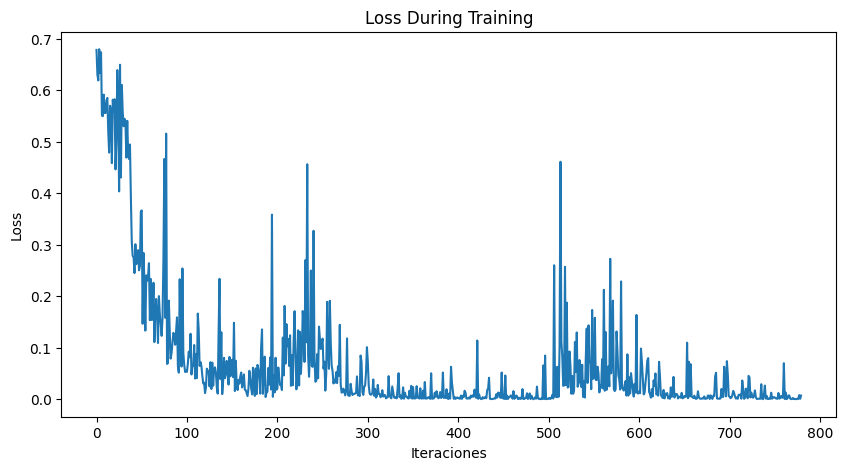
\includegraphics[width=0.85\textwidth]{4/figures/model9_train.PNG}
		\caption[Proceso de entrenamiento del modelo n°9]{Proceso de entrenamiento del modelo n°9. \\
		Fuente: Elaboración propia.}
		\label{4:fig136}
	\end{center}
\end{figure}

También se calcularon su Accuracy, Recall y Precision. Estos son presentados en la Tabla \ref{4:table10}.

\begin{table}[H]
	\caption[Accuracy, Recall y Precision del modelo n°9]{Accuracy, Recall y Precision del modelo n°9.}
	\label{4:table10}
	\centering
	\small
	\begin{tabular}{c|ccc}
		\specialrule{.1em}{.05em}{.05em}
		{Métrica} & {Accuracy} & {Recall} & {Precision} \\
		\hline
		{Valor} & {72.48\%} & {58.90\%} & {65.88\%} \\
		\specialrule{.1em}{.05em}{.05em}
	\end{tabular}
	\begin{flushleft}	
		\small Fuente: Elaboración propia.
	\end{flushleft}
\end{table}

\begin{comment}
\begin{figure}[H]
	\begin{center}
		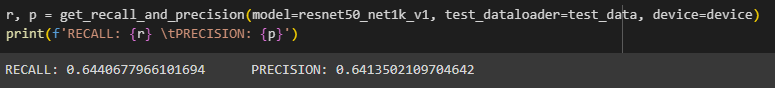
\includegraphics[width=0.83\textwidth]{4/figures/model9_rp.PNG}
		\caption[Recall y Precision del modelo n°9]{Recall y Precision del modelo n°9. \\
		Fuente: Elaboración propia.}
		\label{4:fig137}
	\end{center}
\end{figure}
\end{comment}

El modelo n°10 empleó la técnica de entrenamiento de Transfer Learning  junto con el modelo RESNET50 con pesos de IMAGENET1KV1.

Se presenta en la Figura \ref{4:fig138} el proceso del entrenamiento del modelo RESNET50 con los pesos IMAGENET1KV1 y usando la técnica de Transfer Learning.

\begin{figure}[H]
	\begin{center}
		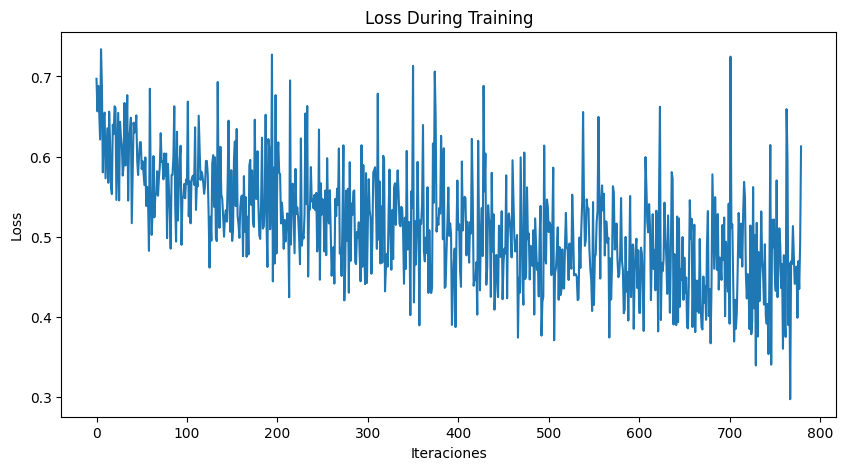
\includegraphics[width=0.85\textwidth]{4/figures/model10_train.PNG}
		\caption[Proceso de entrenamiento del modelo n°10]{Proceso de entrenamiento del modelo n°10. \\
		Fuente: Elaboración propia.}
		\label{4:fig138}
	\end{center}
\end{figure}

También se calcularon su Accuracy, Recall y Precision. Estos son presentados en la Tabla \ref{4:table11}.

\begin{table}[H]
	\caption[Accuracy, Recall y Precision del modelo n°10]{Accuracy, Recall y Precision del modelo n°10.}
	\label{4:table11}
	\centering
	\small
	\begin{tabular}{c|ccc}
		\specialrule{.1em}{.05em}{.05em}
		{Métrica} & {Accuracy} & {Recall} & {Precision} \\
		\hline
		{Valor} & {62.38\%} & {37.71\%} & {51.45\%} \\
		\specialrule{.1em}{.05em}{.05em}
	\end{tabular}
	\begin{flushleft}	
		\small Fuente: Elaboración propia.
	\end{flushleft}
\end{table}

\begin{comment}
\begin{figure}[H]
	\begin{center}
		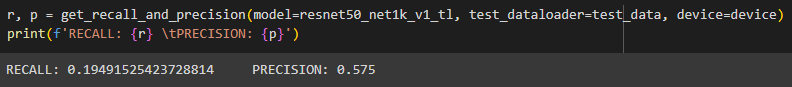
\includegraphics[width=0.83\textwidth]{4/figures/model10_rp.PNG}
		\caption[Recall y Precision del modelo n°10]{Recall y Precision del modelo n°10. \\
		Fuente: Elaboración propia.}
		\label{4:fig139}
	\end{center}
\end{figure}
\end{comment}

El modelo n°11 empleó la técnica de entrenamiento de Fine Tuning junto con el modelo RESNET50 con pesos de IMAGENET1KV2.

Se presenta en la Figura \ref{4:fig140} el proceso del entrenamiento del modelo RESNET50 con los pesos IMAGENET1KV2 y usando la técnica de Fine Tuning.

\begin{figure}[H]
	\begin{center}
		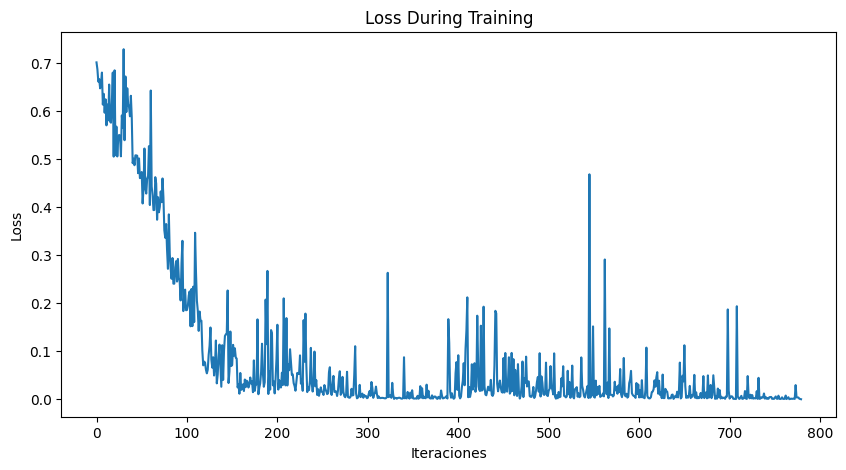
\includegraphics[width=0.85\textwidth]{4/figures/model11_train.PNG}
		\caption[Proceso de entrenamiento del modelo n°11]{Proceso de entrenamiento del modelo n°11. \\
		Fuente: Elaboración propia.}
		\label{4:fig140}
	\end{center}
\end{figure}

También se calcularon su Accuracy, Recall y Precision. Estos son presentados en la Tabla \ref{4:table12}.

\begin{table}[H]
	\caption[Accuracy, Recall y Precision del modelo n°11]{Accuracy, Recall y Precision del modelo n°11.}
	\label{4:table12}
	\centering
	\small
	\begin{tabular}{c|ccc}
		\specialrule{.1em}{.05em}{.05em}
		{Métrica} & {Accuracy} & {Recall} & {Precision} \\
		\hline
		{Valor} & {67.59\%} & {51.27\%} & {59.02\%} \\
		\specialrule{.1em}{.05em}{.05em}
	\end{tabular}
	\begin{flushleft}	
		\small Fuente: Elaboración propia.
	\end{flushleft}
\end{table}

\begin{comment}
\begin{figure}[H]
	\begin{center}
		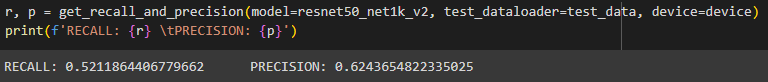
\includegraphics[width=0.83\textwidth]{4/figures/model11_rp.PNG}
		\caption[Recall y Precision del modelo n°11]{Recall y Precision del modelo n°11. \\
		Fuente: Elaboración propia.}
		\label{4:fig141}
	\end{center}
\end{figure}
\end{comment}

El modelo n°12 empleó la técnica de entrenamiento de Transfer Learning junto con el modelo RESNET50 con pesos de IMAGENET1KV2.

Se presenta en la Figura \ref{4:fig142} el proceso del entrenamiento del modelo RESNET50 con los pesos IMAGENET1KV2 y usando la técnica de Transfer Learning.

\begin{figure}[H]
	\begin{center}
		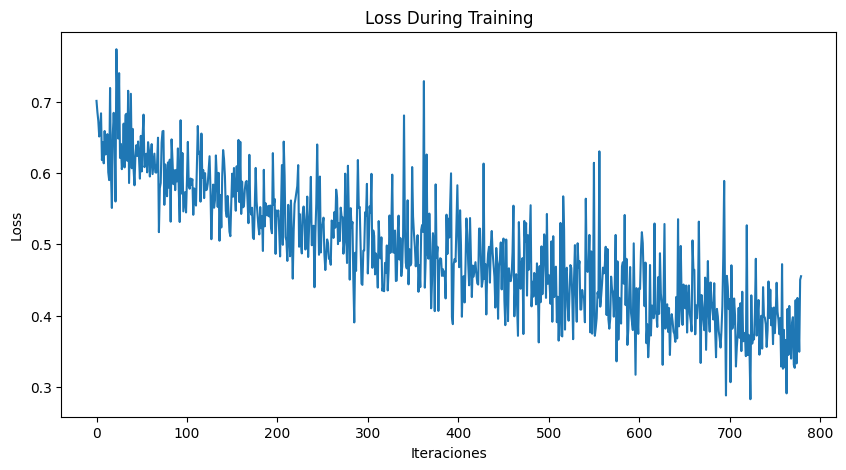
\includegraphics[width=0.85\textwidth]{4/figures/model12_train.PNG}
		\caption[Proceso de entrenamiento del modelo n°12]{Proceso de entrenamiento del modelo n°12. \\
		Fuente: Elaboración propia.}
		\label{4:fig142}
	\end{center}
\end{figure}

También se calcularon su Accuracy, Recall y Precision. Estos son presentados en la Tabla \ref{4:table13}.

\begin{table}[H]
	\caption[Accuracy, Recall y Precision del modelo n°12]{Accuracy, Recall y Precision del modelo n°12.}
	\label{4:table13}
	\centering
	\small
	\begin{tabular}{c|ccc}
		\specialrule{.1em}{.05em}{.05em}
		{Métrica} & {Accuracy} & {Recall} & {Precision} \\
		\hline
		{Valor} & {62.05\%} & {49.15\%} & {50.66\%} \\
		\specialrule{.1em}{.05em}{.05em}
	\end{tabular}
	\begin{flushleft}	
		\small Fuente: Elaboración propia.
	\end{flushleft}
\end{table}

\begin{comment}
\begin{figure}[H]
	\begin{center}
		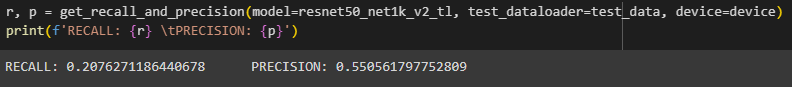
\includegraphics[width=0.83\textwidth]{4/figures/model12_rp.PNG}
		\caption[Recall y Precision del modelo n°12]{Recall y Precision del modelo n°12. \\
		Fuente: Elaboración propia.}
		\label{4:fig143}
	\end{center}
\end{figure}
\end{comment}

Una vez culminado el entrenamiento de los modelos con el conjunto de datos sin imágenes generadas, se inició un nuevo proceso de entrenamiento, esta vez con el conjunto de datos aumentado. 

Todos los modelos, tanto ViT como CNN, poseen las mismas configuraciones definidas antes, así que no hay necesidad de especificarlo nuevamente.

A continuación se presentan las siguientes Figuras y Tablas donde se muestran todos los resultados de los modelos de manera similar a como se presentó anteriormente.

\begin{figure}[H]
	\begin{center}
		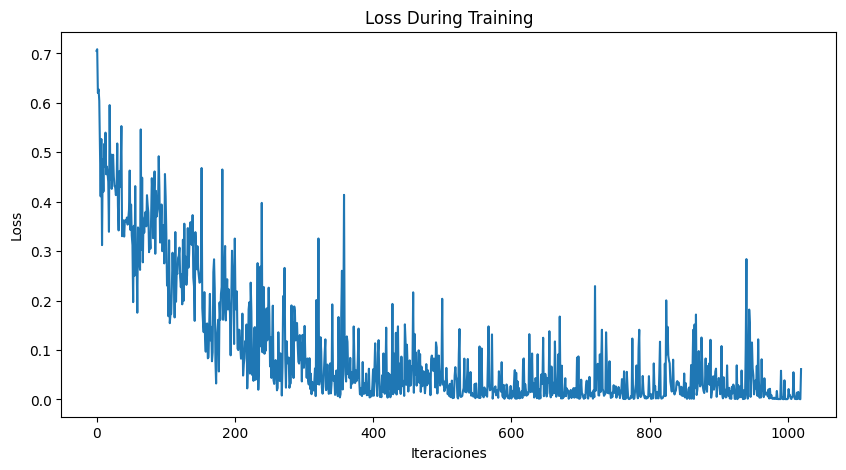
\includegraphics[width=0.85\textwidth]{4/figures/model13_train.PNG}
		\caption[Proceso de entrenamiento del modelo n°13]{Proceso de entrenamiento del modelo n°13. \\
		Fuente: Elaboración propia.}
		\label{4:fig144}
	\end{center}
\end{figure}

\begin{table}[H]
	\caption[Accuracy, Recall y Precision del modelo n°13]{Accuracy, Recall y Precision del modelo n°13.}
	\label{4:table14}
	\centering
	\small
	\begin{tabular}{c|ccc}
		\specialrule{.1em}{.05em}{.05em}
		{Métrica} & {Accuracy} & {Recall} & {Precision} \\
		\hline
		{Valor} & {70.36\%} & {61.44\%} & {61.44\%} \\
		\specialrule{.1em}{.05em}{.05em}
	\end{tabular}
	\begin{flushleft}	
		\small Fuente: Elaboración propia.
	\end{flushleft}
\end{table}

\begin{comment}
\begin{figure}[H]
	\begin{center}
		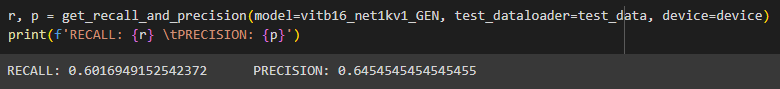
\includegraphics[width=0.83\textwidth]{4/figures/model13_rp.PNG}
		\caption[Recall y Precision del modelo n°13]{Recall y Precision del modelo n°13. \\
		Fuente: Elaboración propia.}
		\label{4:fig145}
	\end{center}
\end{figure}
\end{comment}

\begin{figure}[H]
	\begin{center}
		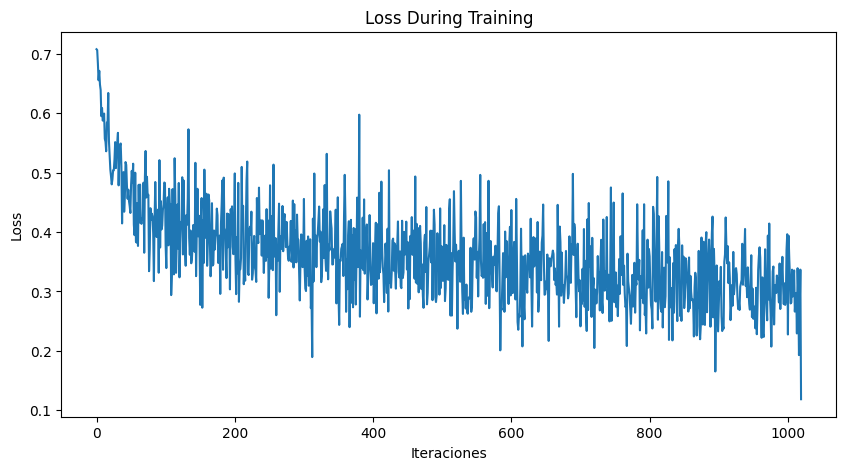
\includegraphics[width=0.85\textwidth]{4/figures/model14_train.PNG}
		\caption[Proceso de entrenamiento del modelo n°14]{Proceso de entrenamiento del modelo n°14. \\
		Fuente: Elaboración propia.}
		\label{4:fig146}
	\end{center}
\end{figure}

\begin{table}[H]
	\caption[Accuracy, Recall y Precision del modelo n°14]{Accuracy, Recall y Precision del modelo n°14.}
	\label{4:table15}
	\centering
	\small
	\begin{tabular}{c|ccc}
		\specialrule{.1em}{.05em}{.05em}
		{Métrica} & {Accuracy} & {Recall} & {Precision} \\
		\hline
		{Valor} & {69.06\%} & {50.00\%} & {62.11\%} \\
		\specialrule{.1em}{.05em}{.05em}
	\end{tabular}
	\begin{flushleft}	
		\small Fuente: Elaboración propia.
	\end{flushleft}
\end{table}

\begin{comment}
\begin{figure}[H]
	\begin{center}
		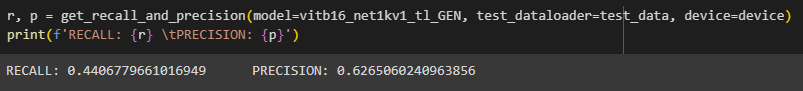
\includegraphics[width=0.83\textwidth]{4/figures/model14_rp.PNG}
		\caption[Recall y Precision del modelo n°14]{Recall y Precision del modelo n°14. \\
		Fuente: Elaboración propia.}
		\label{4:fig147}
	\end{center}
\end{figure}
\end{comment}

\begin{figure}[H]
	\begin{center}
		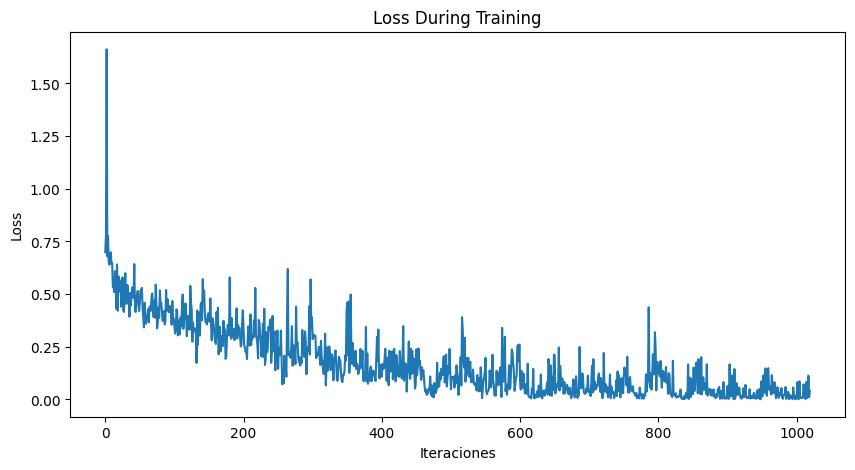
\includegraphics[width=0.85\textwidth]{4/figures/model15_train.PNG}
		\caption[Proceso de entrenamiento del modelo n°15]{Proceso de entrenamiento del modelo n°15. \\
		Fuente: Elaboración propia.}
		\label{4:fig148}
	\end{center}
\end{figure}

\begin{table}[H]
	\caption[Accuracy, Recall y Precision del modelo n°15]{Accuracy, Recall y Precision del modelo n°15.}
	\label{4:table16}
	\centering
	\small
	\begin{tabular}{c|ccc}
		\specialrule{.1em}{.05em}{.05em}
		{Métrica} & {Accuracy} & {Recall} & {Precision} \\
		\hline
		{Valor} & {67.43\%} & {41.10\%} & {61.39\%} \\
		\specialrule{.1em}{.05em}{.05em}
	\end{tabular}
	\begin{flushleft}	
		\small Fuente: Elaboración propia.
	\end{flushleft}
\end{table}

\begin{comment}
\begin{figure}[H]
	\begin{center}
		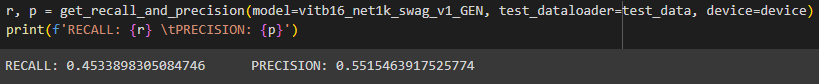
\includegraphics[width=0.83\textwidth]{4/figures/model15_rp.PNG}
		\caption[Recall y Precision del modelo n°15]{Recall y Precision del modelo n°15. \\
		Fuente: Elaboración propia.}
		\label{4:fig149}
	\end{center}
\end{figure}
\end{comment}

\begin{figure}[H]
	\begin{center}
		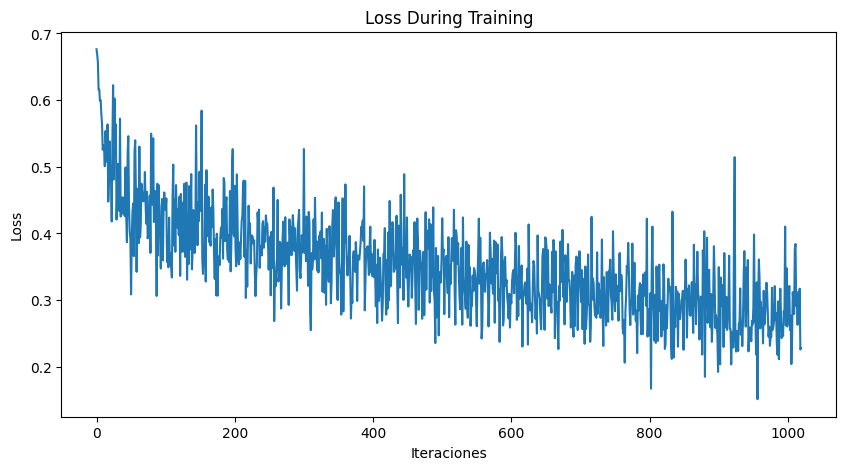
\includegraphics[width=0.85\textwidth]{4/figures/model16_train.PNG}
		\caption[Proceso de entrenamiento del modelo n°16]{Proceso de entrenamiento del modelo n°16. \\
		Fuente: Elaboración propia.}
		\label{4:fig150}
	\end{center}
\end{figure}

\begin{table}[H]
	\caption[Accuracy, Recall y Precision del modelo n°16]{Accuracy, Recall y Precision del modelo n°16.}
	\label{4:table17}
	\centering
	\small
	\begin{tabular}{c|ccc}
		\specialrule{.1em}{.05em}{.05em}
		{Métrica} & {Accuracy} & {Recall} & {Precision} \\
		\hline
		{Valor} & {69.71\%} & {64.83\%} & {59.77\%} \\
		\specialrule{.1em}{.05em}{.05em}
	\end{tabular}
	\begin{flushleft}	
		\small Fuente: Elaboración propia.
	\end{flushleft}
\end{table}

\begin{comment}
\begin{figure}[H]
	\begin{center}
		\includegraphics[width=0.83\textwidth]{4/figures/model16_rp.PNG}
		\caption[Recall y Precision del modelo n°16]{Recall y Precision del modelo n°16. \\
		Fuente: Elaboración propia.}
		\label{4:fig151}
	\end{center}
\end{figure}
\end{comment}

\begin{figure}[H]
	\begin{center}
		\includegraphics[width=0.85\textwidth]{4/figures/model17_train.PNG}
		\caption[Proceso de entrenamiento del modelo n°17]{Proceso de entrenamiento del modelo n°17. \\
		Fuente: Elaboración propia.}
		\label{4:fig152}
	\end{center}
\end{figure}

\begin{table}[H]
	\caption[Accuracy, Recall y Precision del modelo n°17]{Accuracy, Recall y Precision del modelo n°17.}
	\label{4:table18}
	\centering
	\small
	\begin{tabular}{c|ccc}
		\specialrule{.1em}{.05em}{.05em}
		{Métrica} & {Accuracy} & {Recall} & {Precision} \\
		\hline
		{Valor} & {57.65\%} & {41.95\%} & {44.59\%} \\
		\specialrule{.1em}{.05em}{.05em}
	\end{tabular}
	\begin{flushleft}	
		\small Fuente: Elaboración propia.
	\end{flushleft}
\end{table}

\begin{comment}
\begin{figure}[H]
	\begin{center}
		\includegraphics[width=0.83\textwidth]{4/figures/model17_rp.PNG}
		\caption[Recall y Precision del modelo n°17]{Recall y Precision del modelo n°17. \\
		Fuente: Elaboración propia.}
		\label{4:fig153}
	\end{center}
\end{figure}
\end{comment}

\begin{figure}[H]
	\begin{center}
		\includegraphics[width=0.85\textwidth]{4/figures/model18_train.PNG}
		\caption[Proceso de entrenamiento del modelo n°18]{Proceso de entrenamiento del modelo n°18. \\
		Fuente: Elaboración propia.}
		\label{4:fig154}
	\end{center}
\end{figure}

\begin{table}[H]
	\caption[Accuracy, Recall y Precision del modelo n°18]{Accuracy, Recall y Precision del modelo n°18.}
	\label{4:table19}
	\centering
	\small
	\begin{tabular}{c|ccc}
		\specialrule{.1em}{.05em}{.05em}
		{Métrica} & {Accuracy} & {Recall} & {Precision} \\
		\hline
		{Valor} & {64.82\%} & {49.58\%} & {54.67\%} \\
		\specialrule{.1em}{.05em}{.05em}
	\end{tabular}
	\begin{flushleft}	
		\small Fuente: Elaboración propia.
	\end{flushleft}
\end{table}

\begin{comment}
\begin{figure}[H]
	\begin{center}
		\includegraphics[width=0.83\textwidth]{4/figures/model18_rp.PNG}
		\caption[Recall y Precision del modelo n°18]{Recall y Precision del modelo n°18. \\
		Fuente: Elaboración propia.}
		\label{4:fig155}
	\end{center}
\end{figure}
\end{comment}

\begin{figure}[H]
	\begin{center}
		\includegraphics[width=0.85\textwidth]{4/figures/model19_train.PNG}
		\caption[Proceso de entrenamiento del modelo n°19]{Proceso de entrenamiento del modelo n°19. \\
		Fuente: Elaboración propia.}
		\label{4:fig156}
	\end{center}
\end{figure}

\begin{table}[H]
	\caption[Accuracy, Recall y Precision del modelo n°19]{Accuracy, Recall y Precision del modelo n°19.}
	\label{4:table20}
	\centering
	\small
	\begin{tabular}{c|ccc}
		\specialrule{.1em}{.05em}{.05em}
		{Métrica} & {Accuracy} & {Recall} & {Precision} \\
		\hline
		{Valor} & {71.99\%} & {59.75\%} & {64.68\%} \\
		\specialrule{.1em}{.05em}{.05em}
	\end{tabular}
	\begin{flushleft}	
		\small Fuente: Elaboración propia.
	\end{flushleft}
\end{table}

\begin{comment}
\begin{figure}[H]
	\begin{center}
		\includegraphics[width=0.83\textwidth]{4/figures/model19_rp.PNG}
		\caption[Recall y Precision del modelo n°19]{Recall y Precision del modelo n°19. \\
		Fuente: Elaboración propia.}
		\label{4:fig157}
	\end{center}
\end{figure}
\end{comment}

\begin{figure}[H]
	\begin{center}
		\includegraphics[width=0.85\textwidth]{4/figures/model20_train.PNG}
		\caption[Proceso de entrenamiento del modelo n°20]{Proceso de entrenamiento del modelo n°20. \\
		Fuente: Elaboración propia.}
		\label{4:fig158}
	\end{center}
\end{figure}

\begin{table}[H]
	\caption[Accuracy, Recall y Precision del modelo n°20]{Accuracy, Recall y Precision del modelo n°20.}
	\label{4:table21}
	\centering
	\small
	\begin{tabular}{c|ccc}
		\specialrule{.1em}{.05em}{.05em}
		{Métrica} & {Accuracy} & {Recall} & {Precision} \\
		\hline
		{Valor} & {66.45\%} & {52.97\%} & {56.82\%} \\
		\specialrule{.1em}{.05em}{.05em}
	\end{tabular}
	\begin{flushleft}	
		\small Fuente: Elaboración propia.
	\end{flushleft}
\end{table}

\begin{comment}
\begin{figure}[H]
	\begin{center}
		\includegraphics[width=0.83\textwidth]{4/figures/model20_rp.PNG}
		\caption[Recall y Precision del modelo n°20]{Recall y Precision del modelo n°20. \\
		Fuente: Elaboración propia.}
		\label{4:fig159}
	\end{center}
\end{figure}
\end{comment}

\begin{figure}[H]
	\begin{center}
		\includegraphics[width=0.85\textwidth]{4/figures/model21_train.PNG}
		\caption[Proceso de entrenamiento del modelo n°21]{Proceso de entrenamiento del modelo n°21. \\
		Fuente: Elaboración propia.}
		\label{4:fig160}
	\end{center}
\end{figure}

\begin{table}[H]
	\caption[Accuracy, Recall y Precision del modelo n°21]{Accuracy, Recall y Precision del modelo n°21.}
	\label{4:table22}
	\centering
	\small
	\begin{tabular}{c|ccc}
		\specialrule{.1em}{.05em}{.05em}
		{Métrica} & {Accuracy} & {Recall} & {Precision} \\
		\hline
		{Valor} & {70.85\%} & {68.22\%} & {60.75\%} \\
		\specialrule{.1em}{.05em}{.05em}
	\end{tabular}
	\begin{flushleft}	
		\small Fuente: Elaboración propia.
	\end{flushleft}
\end{table}

\begin{comment}
\begin{figure}[H]
	\begin{center}
		\includegraphics[width=0.83\textwidth]{4/figures/model21_rp.PNG}
		\caption[Recall y Precision del modelo n°21]{Recall y Precision del modelo n°21. \\
		Fuente: Elaboración propia.}
		\label{4:fig161}
	\end{center}
\end{figure}
\end{comment}

\begin{figure}[H]
	\begin{center}
		\includegraphics[width=0.85\textwidth]{4/figures/model22_train.PNG}
		\caption[Proceso de entrenamiento del modelo n°22]{Proceso de entrenamiento del modelo n°22. \\
		Fuente: Elaboración propia.}
		\label{4:fig162}
	\end{center}
\end{figure}

\begin{table}[H]
	\caption[Accuracy, Recall y Precision del modelo n°22]{Accuracy, Recall y Precision del modelo n°22.}
	\label{4:table23}
	\centering
	\small
	\begin{tabular}{c|ccc}
		\specialrule{.1em}{.05em}{.05em}
		{Métrica} & {Accuracy} & {Recall} & {Precision} \\
		\hline
		{Valor} & {64.17\%} & {33.90\%} & {55.56\%} \\
		\specialrule{.1em}{.05em}{.05em}
	\end{tabular}
	\begin{flushleft}	
		\small Fuente: Elaboración propia.
	\end{flushleft}
\end{table}

\begin{comment}
\begin{figure}[H]
	\begin{center}
		\includegraphics[width=0.83\textwidth]{4/figures/model22_rp.PNG}
		\caption[Recall y Precision del modelo n°22]{Recall y Precision del modelo n°22. \\
		Fuente: Elaboración propia.}
		\label{4:fig163}
	\end{center}
\end{figure}
\end{comment}

\begin{figure}[H]
	\begin{center}
		\includegraphics[width=0.85\textwidth]{4/figures/model23_train.PNG}
		\caption[Proceso de entrenamiento del modelo n°23]{Proceso de entrenamiento del modelo n°23. \\
		Fuente: Elaboración propia.}
		\label{4:fig164}
	\end{center}
\end{figure}

\begin{table}[H]
	\caption[Accuracy, Recall y Precision del modelo n°23]{Accuracy, Recall y Precision del modelo n°23.}
	\label{4:table24}
	\centering
	\small
	\begin{tabular}{c|ccc}
		\specialrule{.1em}{.05em}{.05em}
		{Métrica} & {Accuracy} & {Recall} & {Precision} \\
		\hline
		{Valor} & {67.92\%} & {55.51\%} & {58.74\%} \\
		\specialrule{.1em}{.05em}{.05em}
	\end{tabular}
	\begin{flushleft}	
		\small Fuente: Elaboración propia.
	\end{flushleft}
\end{table}

\begin{comment}
\begin{figure}[H]
	\begin{center}
		\includegraphics[width=0.83\textwidth]{4/figures/model23_rp.PNG}
		\caption[Recall y Precision del modelo n°23]{Recall y Precision del modelo n°23. \\
		Fuente: Elaboración propia.}
		\label{4:fig165}
	\end{center}
\end{figure}
\end{comment}

\begin{figure}[H]
	\begin{center}
		\includegraphics[width=0.85\textwidth]{4/figures/model24_train.PNG}
		\caption[Proceso de entrenamiento del modelo n°24]{Proceso de entrenamiento del modelo n°24. \\
		Fuente: Elaboración propia.}
		\label{4:fig166}
	\end{center}
\end{figure}

\begin{table}[H]
	\caption[Accuracy, Recall y Precision del modelo n°24]{Accuracy, Recall y Precision del modelo n°24.}
	\label{4:table25}
	\centering
	\small
	\begin{tabular}{c|ccc}
		\specialrule{.1em}{.05em}{.05em}
		{Métrica} & {Accuracy} & {Recall} & {Precision} \\
		\hline
		{Valor} & {62.87\%} & {47.03\%} & {51.87\%} \\
		\specialrule{.1em}{.05em}{.05em}
	\end{tabular}
	\begin{flushleft}	
		\small Fuente: Elaboración propia.
	\end{flushleft}
\end{table}

\begin{comment}
\begin{figure}[H]
	\begin{center}
		\includegraphics[width=0.83\textwidth]{4/figures/model24_rp.PNG}
		\caption[Recall y Precision del modelo n°24]{Recall y Precision del modelo n°24. \\
		Fuente: Elaboración propia.}
		\label{4:fig167}
	\end{center}
\end{figure}
\end{comment}

\textbf{Actividad 3:  Definir modelos híbridos entre ViT y CNN}
\\
Luego del entrenamiento y un análisis rápido de resultados de los modelos CNN y ViT, se determinó que la arquitectura de mejor desempeño fue ResNet50 con los pesos de IMAGENET1KV1 entrenado con la técnica de Fine Tuning y sin la data aumentada, pues su métrica Accuracy superó a los demás modelos. En segundo lugar se ubica el modelo VGG16 con los pesos de IMAGENET1KV1 entrenado con la técnica de Fine Tuning y sin la data aumentada.

Se decidió tomar ambos modelos CNN para la construcción de modelos híbridos con ViT. Para lograr esto, se usó la librería “transformers” de Python que se encuentra actualmente mantenida por Hugging Face. Esta librería permitió personalizar un modelo ViT híbrido base, lo cuál facilitó su construcción, a diferencia de las herramientas incluidas en mismo Pytorch, específicamente Torchvision, donde los modelos ViT venían de forma predefinida y dificultaban su personalización de acuerdo a las necesidades de esta investigación.

Es así que, para lograr un correcta integración de los modelos ResNet50 y VGG16 con ViT, fue necesario configurar todos los híbridos con un nuevo tamaño de features que recibirá la arquitectura ViT dependiendo del tipo de backbone, además, el tamaño de la imagen de entrada fue establecida a 128 x 128. El tamaño de patch se estableció en 1 (valor por defecto en la creación del modelo) de igual forma a cómo se define el paper de \cite{pr_JERBI2023autoclassViTGAN} que fue fuente original y de inspiración para esta investigación. Finalmente, se configuró el bloque clasificador del ViT a un MLP con dos capas de configuración (256, 1) y con una función de activación ReLU en la primera de estas.

De forma adicional, se usó el modelo híbrido desarrollado por Google y preentrando con el conjunto de datos IMAGENET21K: ViT-hybrid-base-bit-384. Este modelo usa como backbone una versión modificada de las arquitecturas ResNet. Para lograr adaptarlo a la tarea de esta investigación, se modificó su bloque clasificador a un MLP con una sola capa de una neurona.

\textbf{Actividad 4: Entrenar y probar modelos híbridos CNN + ViT}
\\
Ya con los modelos híbridos construidos se pasó a la etapa de entrenamiento.

Debido a que los modelos CNN ResNet50 y VGG16 de mayor desempeño se entrenaron con los pesos de IMAGENET1KV1 con Fine Tuning y sin la data aumentada, se usó esta misma configuración para los modelos híbridos. De igual forma, la función de pérdida y de optimización se mantuvieron como los anteriores modelos.

En el caso del modelo híbrido de Google, la única diferencia fue que se estableció el tamaño de lote a 32 debido a las limitaciones de hardware.

Con todas esta especificaciones, se inició el entrenamiento de los modelos híbridos con 20 épocas. 

A continuación, en la Figura \ref{4:fig168} se presenta el proceso de entrenamiento del modelo híbrido ViT + ResNet50 con los pesos pre-entrenados de IMAGENET1KV1 y el tipo de entrenamiento Fine Tuning.

\begin{figure}[H]
	\begin{center}
		\includegraphics[width=0.85\textwidth]{4/figures/modelH_resnet_train.PNG}
		\caption[Proceso de entrenamiento del modelo híbrido ViT + ResNet50]{Proceso de entrenamiento del modelo híbrido ViT + ResNet50. \\
		Fuente: Elaboración propia.}
		\label{4:fig168}
	\end{center}
\end{figure}


Además, también se presenta las métricas de Accuracy, Recall y Precision en la Tabla \ref{4:table26}.

\begin{table}[H]
	\caption[Accuracy, Recall y Precision del modelo híbrido ViT + ResNet50]{Accuracy, Recall y Precision del modelo híbrido ViT + ResNet50.}
	\label{4:table26}
	\centering
	\small
	\begin{tabular}{c|ccc}
		\specialrule{.1em}{.05em}{.05em}
		{Métrica} & {Accuracy} & {Recall} & {Precision} \\
		\hline
		{Valor} & {57.00\%} & {48.73\%} & {44.57\%} \\
		\specialrule{.1em}{.05em}{.05em}
	\end{tabular}
	\begin{flushleft}	
		\small Fuente: Elaboración propia.
	\end{flushleft}
\end{table}

De igual manera, en la Figura \ref{4:fig172} se presenta el proceso de entrenamiento del modelo híbrido ViT + VGG16 con los pesos pre-entrenados de IMAGENET1KV1 y el tipo de entrenamiento Fine Tuning.

\begin{figure}[H]
	\begin{center}
		\includegraphics[width=0.85\textwidth]{4/figures/modelH_vgg_train.PNG}
		\caption[Proceso de entrenamiento del modelo híbrido ViT + VGG16]{Proceso de entrenamiento del modelo híbrido ViT + VGG16. \\
		Fuente: Elaboración propia.}
		\label{4:fig172}
	\end{center}
\end{figure}

Se presenta las métricas de Accuracy, Recall y Precision en la Tabla \ref{4:table30}.

\begin{table}[H]
	\caption[Accuracy, Recall y Precision del modelo híbrido ViT + VGG16]{Accuracy, Recall y Precision del modelo híbrido ViT + VGG16.}
	\label{4:table30}
	\centering
	\small
	\begin{tabular}{c|ccc}
		\specialrule{.1em}{.05em}{.05em}
		{Métrica} & {Accuracy} & {Recall} & {Precision} \\
		\hline
		{Valor} & {55.37\%} & {44.49\%} & {42.34\%} \\
		\specialrule{.1em}{.05em}{.05em}
	\end{tabular}
	\begin{flushleft}	
		\small Fuente: Elaboración propia.
	\end{flushleft}
\end{table}

Finalmente, en la Figura \ref{4:fig173} se presenta el proceso de entrenamiento del modelo híbrido de Google con los pesos pre-entrenados de IMAGENET21k y el tipo de entrenamiento Fine Tuning.

\begin{figure}[H]
	\begin{center}
		\includegraphics[width=0.85\textwidth]{4/figures/modelH_google_train.PNG}
		\caption[Proceso de entrenamiento del modelo híbrido de Google]{Proceso de entrenamiento del modelo híbrido de Google. \\
		Fuente: Elaboración propia.}
		\label{4:fig173}
	\end{center}
\end{figure}

Se presenta las métricas de Accuracy, Recall y Precision en la Tabla \ref{4:table31}.

\begin{table}[H]
	\caption[Accuracy, Recall y Precision del modelo híbrido de Google]{Accuracy, Recall y Precision del modelo híbrido de Google.}
	\label{4:table31}
	\centering
	\small
	\begin{tabular}{c|ccc}
		\specialrule{.1em}{.05em}{.05em}
		{Métrica} & {Accuracy} & {Recall} & {Precision} \\
		\hline
		{Valor} & {77.20\%} & {77.97\%} & {67.65\%} \\
		\specialrule{.1em}{.05em}{.05em}
	\end{tabular}
	\begin{flushleft}	
		\small Fuente: Elaboración propia.
	\end{flushleft}
\end{table}

\section{Medición de la solución}

\subsection{Análisis de Indicadores cuantitativo}
Los indicadores a analizar en esta sección son los obtenidos en el entrenamiento de todos los modelos CNN y ViT, incluyendo además los modelos híbridos. Cada uno de estos dio como resultado principal tres indicadores: Accuracy, Recall y Precision. El primero de estos permitió determinar la capacidad de predicción para ambas clases. El segundo y tercer indicador ayudan a evaluar el modelo en cuestión de capacidad de predicción para la clase positiva. En el caso de esta investigación, la clase positiva es maligno (1).

En la Tabla \ref{4:table1} se presentan los resultados de los modelos.

\begin{table}[H]
	\caption[Resultados de los modelos entrenados con los dos conjuntos de datos, técnicas de entrenamiento y pesos]{Resultados de los modelos entrenados con los dos conjuntos de datos, técnicas de entrenamiento y pesos.}
	\label{4:table1}
	\centering
	\small
	\begin{tabular}{m{2cm}m{2.5cm}m{3cm}m{1.8cm}ccc}
		\specialrule{.1em}{.05em}{.05em}
		{Aumento de datos con DCGAN} & {Modelo} & {Pesos} & {Tipo de entrenamiento} & {Accuracy} & {Recall} & {Precision} \\
		\specialrule{.1em}{.05em}{.05em}
		\multirow{12}{4cm}{No} & \multirow{6}{4cm}{ViT B 16} & \multirow{2}{4cm}{I-NET1K V1} & {FT} & {69.54\%} & {47.03\%} & {64.16\%} \\
		{} & {} & {} & {TL} & {68.08\%} & {53.39\%} & {59.43\%} \\
		{} & {} & \multirow{2}{4cm}{I-NET1K SE V1} & {FT} & {56.84\%} & {53.81\%} & {44.88\%} \\
		{} & {} & {} & {TL} & {69.22\%} & {55.51\%} & {60.93\%} \\
		{} & {} & \multirow{2}{4cm}{I-NET1K SL V1} & {FT} & {58.47\%} & {34.75\%} & {44.81\%} \\
		{} & {} & {} & {TL} & {65.31\%} & {41.95\%} & {56.57\%} \\
		{} & \multirow{2}{4cm}{VGG16} & \multirow{2}{4cm}{I-NET1K V1} & {FT} & {71.99\%} & {58.90\%} & {64.95\%} \\
		{} & {} & {} & {TL} & {65.80\%} & {67.37\%} & {54.45\%} \\
		{} & \multirow{4}{4cm}{RESNET50} & \multirow{2}{4cm}{I-NET1K V1} & {FT} & {72.48\%} & {58.90\%} & {65.88\%} \\
		{} & {} & {} & {TL} & {62.38\%} & {37.71\%} & {51.45\%} \\
		{} & {} & \multirow{2}{4cm}{I-NET1K V2} & {FT} & {67.59\%} & {51.27\%} & {59.02\%} \\
		{} & {} & {} & {TL} & {62.05\%} & {49.15\%} & {50.66\%} \\
		\specialrule{.1em}{.05em}{.05em}
		\multirow{12}{4cm}{Sí} & \multirow{6}{4cm}{ViT B 16} & \multirow{2}{4cm}{I-NET1K V1} & {FT} & {70.36\%} & {61.44\%} & {61.44\%} \\
		{} & {} & {} & {TL} & {69.06\%} & {50.00\%} & {62.11\%} \\
		{} & {} & \multirow{2}{4cm}{I-NET1K SE V1} & {FT} & {67.43\%} & {41.10\%} & {61.39\%} \\
		{} & {} & {} & {TL} & {69.71\%} & {64.83\%} & {59.77\%} \\
		{} & {} & \multirow{2}{4cm}{I-NET1K SL V1} & {FT} & {57.65\%} & {41.95\%} & {44.59\%} \\
		{} & {} & {} & {TL} & {64.82\%} & {49.58\%} & {54.67\%} \\
		{} & \multirow{2}{4cm}{VGG16} & \multirow{2}{4cm}{I-NET1K V1} & {FT} & {71.99\%} & {59.75\%} & {64.68\%} \\
		{} & {} & {} & {TL} & {66.45\%} & {52.97\%} & {56.82\%} \\
		{} & \multirow{4}{4cm}{RESNET50} & \multirow{2}{4cm}{I-NET1K V1} & {FT} & {70.85\%} & {68.22\%} & {60.75\%} \\
		{} & {} & {} & {TL} & {64.17\%} & {33.90\%} & {55.56\%} \\
		{} & {} & \multirow{2}{4cm}{I-NET1K V2} & {FT} & {67.92\%} & {55.51\%} & {58.74\%} \\
		{} & {} & {} & {TL} & {62.87\%} & {47.03\%} & {51.87\%} \\
		\specialrule{.1em}{.05em}{.05em}
		%{No} & {Híbrido} & {I-NET1K V1} & {FT} & {67.92\%} & {78.81\%} & {55.86\%} \\
		{No} & {ViT + ResNet50} & {I-NET1K V1} & {FT} & {57.00\%} & {48.73\%} & {44.57\%} \\
		{No} & {ViT + VGG16} & {I-NET1K V1} & {FT} & {55.37\%} & {44.49\%} & {42.34\%} \\
		{No} & {Híbrido Google} & {I-NET 21k} & {FT} & {\textbf{77.20\%}} & {\textbf{77.97\%}} & {\textbf{67.65\%}} \\
		\specialrule{.1em}{.05em}{.05em}
	\end{tabular}
	\begin{flushleft}	
		\small Fuente: Elaboración propia.
	\end{flushleft}
\end{table}

En relación al indicador Accuracy, el modelo de mejor desempeño fue el modelo híbrido de Google con los pesos IMAGENET21k y la técnica de entrenamiento Fine Tuning, junto con el uso del conjunto de datos original, alcanzado un valor de 77.20\%. En este mismo modelo, las otras dos métricas también fueron los más altos, siendo el caso del Recall (77.97\%) el valor más alto y con un gran margen respecto al Recall de los demás modelos, mientras que el Precision (67.65\%) superó, aunque por menor margen, al segundo mejor modelo en esta métrica.

Algo que mecionar sobre los demás modelos no híbridos es que no hubo una gran diferencia entre los resultados de usar la data aumentada y la origianl, pues el DCGAN no logró capturar al distribución de los imágenes originales, por que su impacto en el entrenamiento no fue tan alto. Esto es debido principalmente a que esta arquitectura fue entrenada con pocos datos (clase minoritaria), lo cuál desencadenó que finalmente las imágenes generadas no tuvieron gran parecido a las originales. 

Debido a la naturaleza del problema de esta investigación, se considera que las métricas de Recall y Precision deben ser relativamente altas para lograr seleccionar el modelo, de igual manera, el Accuracy, que mide la capacidad de predicción para ambar clases, también debe ser alta, ya que es importante determinar no solo si un nódulo es malingo, sino también benigno, ya que esto determinará el tipo de tratamiento posterior que se recomendará a los pacientes. Por este motivo, se decidió elegir el modelo híbrido de Google con los pesos IMAGENET21K y la técnica de entrenamiento Fine Tuning como el modelo para la simulación, ya que posee un Accuracy, Recall y Precision superior a los demás modelos.

\subsection{Simulación de solución}

Luego del análisis de los indicadores de los modelos, y de la elección final, se decidió realizar una simulación de uso del modelo con imágenes del conjunto de datos de prueba.

Para lograr esto, se usó la librería ipywidgets de python que permitió, a través de un mismo jupyter notebook, subir una imagen e ingresarlo al modelo ya cargado y obtener finalmente el resultado de su predicción. En la Figura \ref{4:fig174} se muestra el cargado de las imágenes, mientras que en la Figura \ref{4:fig170} y Figura \ref{4:fig171} se muestra la prueba con dos imágenes de ultrasonido de distintas clases.

\begin{figure}[H]
	\begin{center}
		\includegraphics[width=0.80\textwidth]{4/figures/upload_image.png}
		\caption[Cargado de imágenes de ultrasonido para prueba del modelo]{Cargado de imágenes de ultrasonido para prueba del modelo. \\
		Fuente: Elaboración propia.}
		\label{4:fig174}
	\end{center}
\end{figure}

\begin{figure}[H]
	\begin{center}
		\includegraphics[width=0.58\textwidth]{4/figures/upload_malign.png}
		\caption[Prueba de modelo con imágen de ultrasonido de nódulo maligno]{Prueba de modelo con imágen de ultrasonido de nódulo maligno. \\
		Fuente: Elaboración propia.}
		\label{4:fig170}
	\end{center}
\end{figure}

\begin{figure}[H]
	\begin{center}
		\includegraphics[width=0.58\textwidth]{4/figures/upload_benign.png}
		\caption[Prueba de modelo con imágen de ultrasonido de nódulo benigno]{Prueba de modelo con imágen de ultrasonido de nódulo benigno. \\
		Fuente: Elaboración propia.}
		\label{4:fig171}
	\end{center}
\end{figure}
